%% 
%% Copyright 2007-2020 Elsevier Ltd
%% 
%% This file is part of the 'Elsarticle Bundle'.
%% ---------------------------------------------
%% 
%% It may be distributed under the conditions of the LaTeX Project Public
%% License, either version 1.2 of this license or (at your option) any
%% later version.  The latest version of this license is in
%%    http://www.latex-project.org/lppl.txt
%% and version 1.2 or later is part of all distributions of LaTeX
%% version 1999/12/01 or later.
%% 
%% The list of all files belonging to the 'Elsarticle Bundle' is
%% given in the file `manifest.txt'.
%% 
%% Template article for Elsevier's document class `elsarticle'
%% with harvard style bibliographic references

%\documentclass[preprint,12pt,authoryear]{elsarticle}

%% Use the option review to obtain double line spacing
%% \documentclass[authoryear,preprint,review,12pt]{elsarticle}

%% Use the options 1p,twocolumn; 3p; 3p,twocolumn; 5p; or 5p,twocolumn
%% for a journal layout:
%% \documentclass[final,1p,times,authoryear]{elsarticle}
%% \documentclass[final,1p,times,twocolumn,authoryear]{elsarticle}
%% \documentclass[final,3p,times,authoryear]{elsarticle}
%% \documentclass[final,3p,times,twocolumn,authoryear]{elsarticle}
%% \documentclass[final,5p,times,authoryear]{elsarticle}
 \documentclass[final,5p,times,twocolumn,authoryear,lefttitle]{elsarticle}

%% For including figures, graphicx.sty has been loaded in
%% elsarticle.cls. If you prefer to use the old commands
%% please give \usepackage{epsfig}

%% The amssymb package provides various useful mathematical symbols
\usepackage{amssymb}
\usepackage{amsmath}
\usepackage{lipsum}
\usepackage{sectsty}
\usepackage{placeins}
\sectionfont{\bfseries}
\subsectionfont{\bfseries}
\subsubsectionfont{\bfseries}
%% The amsthm package provides extended theorem environments
%% \usepackage{amsthm}

%% The lineno packages adds line numbers. Start line numbering with
%% \begin{linenumbers}, end it with \end{linenumbers}. Or switch it on
%% for the whole article with \linenumbers.
%% \usepackage{lineno}

%% You might want to define your own abbreviated commands for common used terms, e.g.:
\newcommand{\kms}{km\,s$^{-1}$}
\newcommand{\msun}{$M_\odot}

\journal{Astronomy $\&$ Computing}


\begin{document}

\begin{frontmatter}

%% Title, authors and addresses

%% use the tnoteref command within \title for footnotes;
%% use the tnotetext command for theassociated footnote;
%% use the fnref command within \author or \affiliation for footnotes;
%% use the fntext command for theassociated footnote;
%% use the corref command within \author for corresponding author footnotes;
%% use the cortext command for theassociated footnote;
%% use the ead command for the email address,
%% and the form \ead[url] for the home page:
%% \title{Title\tnoteref{label1}}
%% \tnotetext[label1]{}
%% \author{Name\corref{cor1}\fnref{label2}}
%% \ead{email address}
%% \ead[url]{home page}
%% \fntext[label2]{}
%% \cortext[cor1]{}
%% \affiliation{organization={},
%%            addressline={}, 
%%            city={},
%%            postcode={}, 
%%            state={},
%%            country={}}
%% \fntext[label3]{}

\title{Modelo Predictivo de Riesgo de Desnutrición Crónica Infantil en el Perú mediante Machine Learning}

%% use optional labels to link authors explicitly to addresses:
%% \author[label1,label2]{}
%% \affiliation[label1]{organization={},
%%             addressline={},
%%             city={},
%%             postcode={},
%%             state={},
%%             country={}}
%%
%% \affiliation[label2]{organization={},
%%             addressline={},
%%             city={},
%%             postcode={},
%%             state={},
%%             country={}}

\author[first]{Abel Is-Boset Guevara Huasco}
\author[first]{Zulin Pamela Vallejos Cotrina}
\author[first]{Verónica Lisseth Vergara Rojas}
\affiliation[first]{organization={Escuela Profesional de Ingeniería de Sistemas, Facultad de Ingeniería y Arquitectura, Universidad Peruana Unión}, city={Lima}, country={Perú}}

\begin{abstract}
%% Text of abstract
Example abstract for the astronomy and computing journal. Here you provide a brief summary of the research and the results.
\end{abstract}

%%Graphical abstract
%\begin{graphicalabstract}
%\includegraphics{grabs}
%\end{graphicalabstract}

%%Research highlights
%\begin{highlights}
%\item Research highlight 1
%\item Research highlight 2
%\end{highlights}

\begin{keyword}
%% keywords here, in the form: keyword \sep keyword, up to a maximum of 6 keywords
keyword 1 \sep keyword 2 \sep keyword 3 \sep keyword 4

%% PACS codes here, in the form: \PACS code \sep code

%% MSC codes here, in the form: \MSC code \sep code
%% or \MSC[2008] code \sep code (2000 is the default)

\end{keyword}


\end{frontmatter}

%\tableofcontents

%% \linenumbers

%% main text

\section{Introducción}
\label{introduction}

La desnutrición crónica infantil constituye uno de los principales desafíos de salud pública a nivel mundial, ya que afecta el desarrollo físico, cognitivo y social de millones de niños menores de cinco años [1][2]. Este problema no solo compromete el bienestar y la calidad de vida de la infancia, sino que también limita el progreso económico y social de las naciones, dificultando el cumplimiento del Objetivo de Desarrollo Sostenible 2: Hambre Cero [3]. La desnutrición infantil es un fenómeno complejo, influido por múltiples factores interrelacionados, como las condiciones económicas, la educación materna, el acceso a servicios básicos, la calidad del entorno ambiental y las desigualdades territoriales [4][5]. En el caso del Perú, la desnutrición crónica infantil continúa siendo un problema estructural: según la Encuesta Demográfica y de Salud Familiar (ENDES, 2023), la prevalencia nacional alcanza el 11,5~\%, con regiones como Huancavelica y Loreto que superan el 20~\% [15]. Esta desigualdad evidencia que el problema responde también a factores socioeconómicos, sanitarios y ambientales que varían de forma significativa según el territorio.

Este estudio se justifica desde tres ámbitos complementarios. Desde el ámbito teórico, contribuye al conocimiento existente al incorporar los determinantes sociales, ambientales y espaciales en el análisis de la desnutrición infantil mediante enfoques de machine learning, superando las limitaciones de los modelos estadísticos tradicionales centrados únicamente en variables antropométricas [17][18]. Desde el punto de vista práctico, la propuesta busca desarrollar un sistema de pronóstico geoespacial que permita identificar zonas con mayor probabilidad de riesgo nutricional, de modo que instituciones como el Ministerio de Salud, el MIDIS y los gobiernos regionales puedan priorizar intervenciones preventivas y optimizar la distribución de recursos [16][19][20]. Desde el enfoque innovador, el estudio propone la integración de modelos híbridos de machine learning con análisis geoespacial, un enfoque poco explorado en el contexto peruano y latinoamericano, que ofrece además un marco metodológico replicable para otras problemáticas sociales [21][22].

Durante la última década, diversas investigaciones han empleado métodos estadísticos y de machine learning para analizar la desnutrición infantil, logrando avances significativos en la clasificación del estado nutricional y la identificación de factores asociados. Modelos híbridos y de ensamble, como los propuestos por Alam et al. y Hadikurniawati et al., alcanzaron altos niveles de precisión al integrar variables antropométricas, demográficas y socioeconómicas [8][9]. De forma complementaria, estudios con enfoque espacial, como los de Habtewold et al. y Egbon et al., incorporaron análisis bayesianos y geográficos para identificar zonas críticas y patrones territoriales del riesgo nutricional [10][11]. En África Subsahariana, Backer y Billing desarrollaron un modelo basado en Random Forest para predecir la prevalencia de desnutrición aguda considerando variables ambientales y de conflicto [26], mientras que Tadesse et al. aplicaron un enfoque de Gradient Boosting combinado con señales satelitales, alcanzando un AUC de 0.86 en predicciones a seis meses [27]. En el ámbito del análisis espacial, Aheto et al. propusieron un modelo bayesiano espaciotemporal para estimar la desnutrición crónica en Ghana [28], y Mgomezulu et al. combinaron algoritmos de ensamble con técnicas de balanceo de clases (SMOTE), logrando una precisión del 99~\% en Malawi [13]. Estas experiencias evidencian el creciente potencial de la inteligencia artificial para mejorar el diagnóstico y el pronóstico de la desnutrición infantil, especialmente en contextos donde la información es limitada o dispersa.

A pesar de estos avances, se identifican limitaciones metodológicas específicas que restringen la aplicabilidad y la generalización de los modelos existentes. La mayoría de estos estudios se ha desarrollado en contextos de Asia y África, centrándose en variables antropométricas individuales sin integrar de manera conjunta las dimensiones sociales, ambientales y territoriales [12][14]. Además, el tratamiento combinado de datos espaciales y socioeconómicos presenta dificultades debido a la heterogeneidad de las fuentes, la diferencia en sus escalas y unidades, y la ausencia de técnicas capaces de vincular de manera coherente la información tabular con la información geográfica [11][13]. Por otro lado, los modelos híbridos que integran machine learning y análisis geoespacial se han explorado escasamente en América Latina, región donde las particularidades geográficas y las desigualdades territoriales exigen enfoques adaptados a su propio contexto [32]. En el caso peruano en particular, los estudios nacionales aún no aplican enfoques predictivos ni análisis geoespaciales que permitan anticipar zonas de riesgo [16], lo que evidencia una brecha entre el conocimiento internacional disponible y su aplicación efectiva al contexto local.

Por lo tanto, el presente estudio tiene como objetivo desarrollar un modelo predictivo de riesgo de desnutrición crónica infantil en el Perú mediante machine learning, que permita analizar territorialmente los factores predominantes por departamento y estimar el riesgo nutricional a nivel individual y territorial.

Las contribuciones de este estudio son las siguientes: 1) la depuración y estructuración de una base de datos consistente que integra el estado nutricional infantil a nivel nacional a partir de los microdatos de la ENDES correspondientes al periodo 2007--2024; 2) la comparación sistemática de algoritmos de machine learning (Regresión Logística, Árbol de Decisión, XGBoost, LightGBM, CatBoost y Red Neuronal) bajo un mismo protocolo de validación cruzada estratificada, con el fin de seleccionar el modelo con el mejor desempeño predictivo; 3) la evaluación del modelo mediante métricas de validación (Accuracy, Precision, Recall, F1-score y AUC) y la interpretación de la influencia de las variables mediante valores SHAP, lo que incrementa su capacidad explicativa; y 4) la implementación de un sistema interactivo de análisis territorial que permite visualizar el riesgo de desnutrición según el perfil ingresado, facilitando su aplicación por parte de instituciones públicas de salud [34][37].

Este artículo se organiza de la siguiente manera: la Sección 2 describe la metodología empleada, incluyendo el diseño CRISP-DM, la construcción de la base de datos y el modelo híbrido propuesto. La Sección 3 presenta los resultados obtenidos en la comparación de algoritmos y en la interpretación de variables mediante SHAP. La Sección 4 discute la interpretación de los resultados, su comparación con estudios similares y las limitaciones del estudio. Finalmente, la Sección 5 presenta las conclusiones, replanteando los objetivos, los principales hallazgos y las líneas de trabajo futuro.

\section{Metodología}
\label{metodologia}

La presente investigación se desarrolló bajo el marco CRISP-DM (Cross-Industry Standard Process for Data Mining), organizado en las fases de comprensión de los datos, preparación, modelado, evaluación y despliegue. En primer lugar, se integraron los microdatos de la ENDES y se definió la variable objetivo, aplicando controles para prevenir la fuga de información. A continuación, se armonizaron y preprocesaron los registros, y se seleccionaron las características predictoras. En la fase de modelado se trataron las diferencias de representación muestral y se compararon seis algoritmos supervisados. Luego, el desempeño se evaluó mediante validación cruzada, métricas ponderadas, remuestreo bootstrap y comparación de curvas ROC; las predicciones también se interpretaron con SHAP. Finalmente, se implementó la aplicación de soporte a la decisión y se evaluó su pertinencia con profesionales de salud. El flujo metodológico completo se resume en la Figura~\ref{fig:flujo_metodologico}; las subsecciones siguientes describen estas etapas en ese orden.

\begin{figure*}[t]
\centering
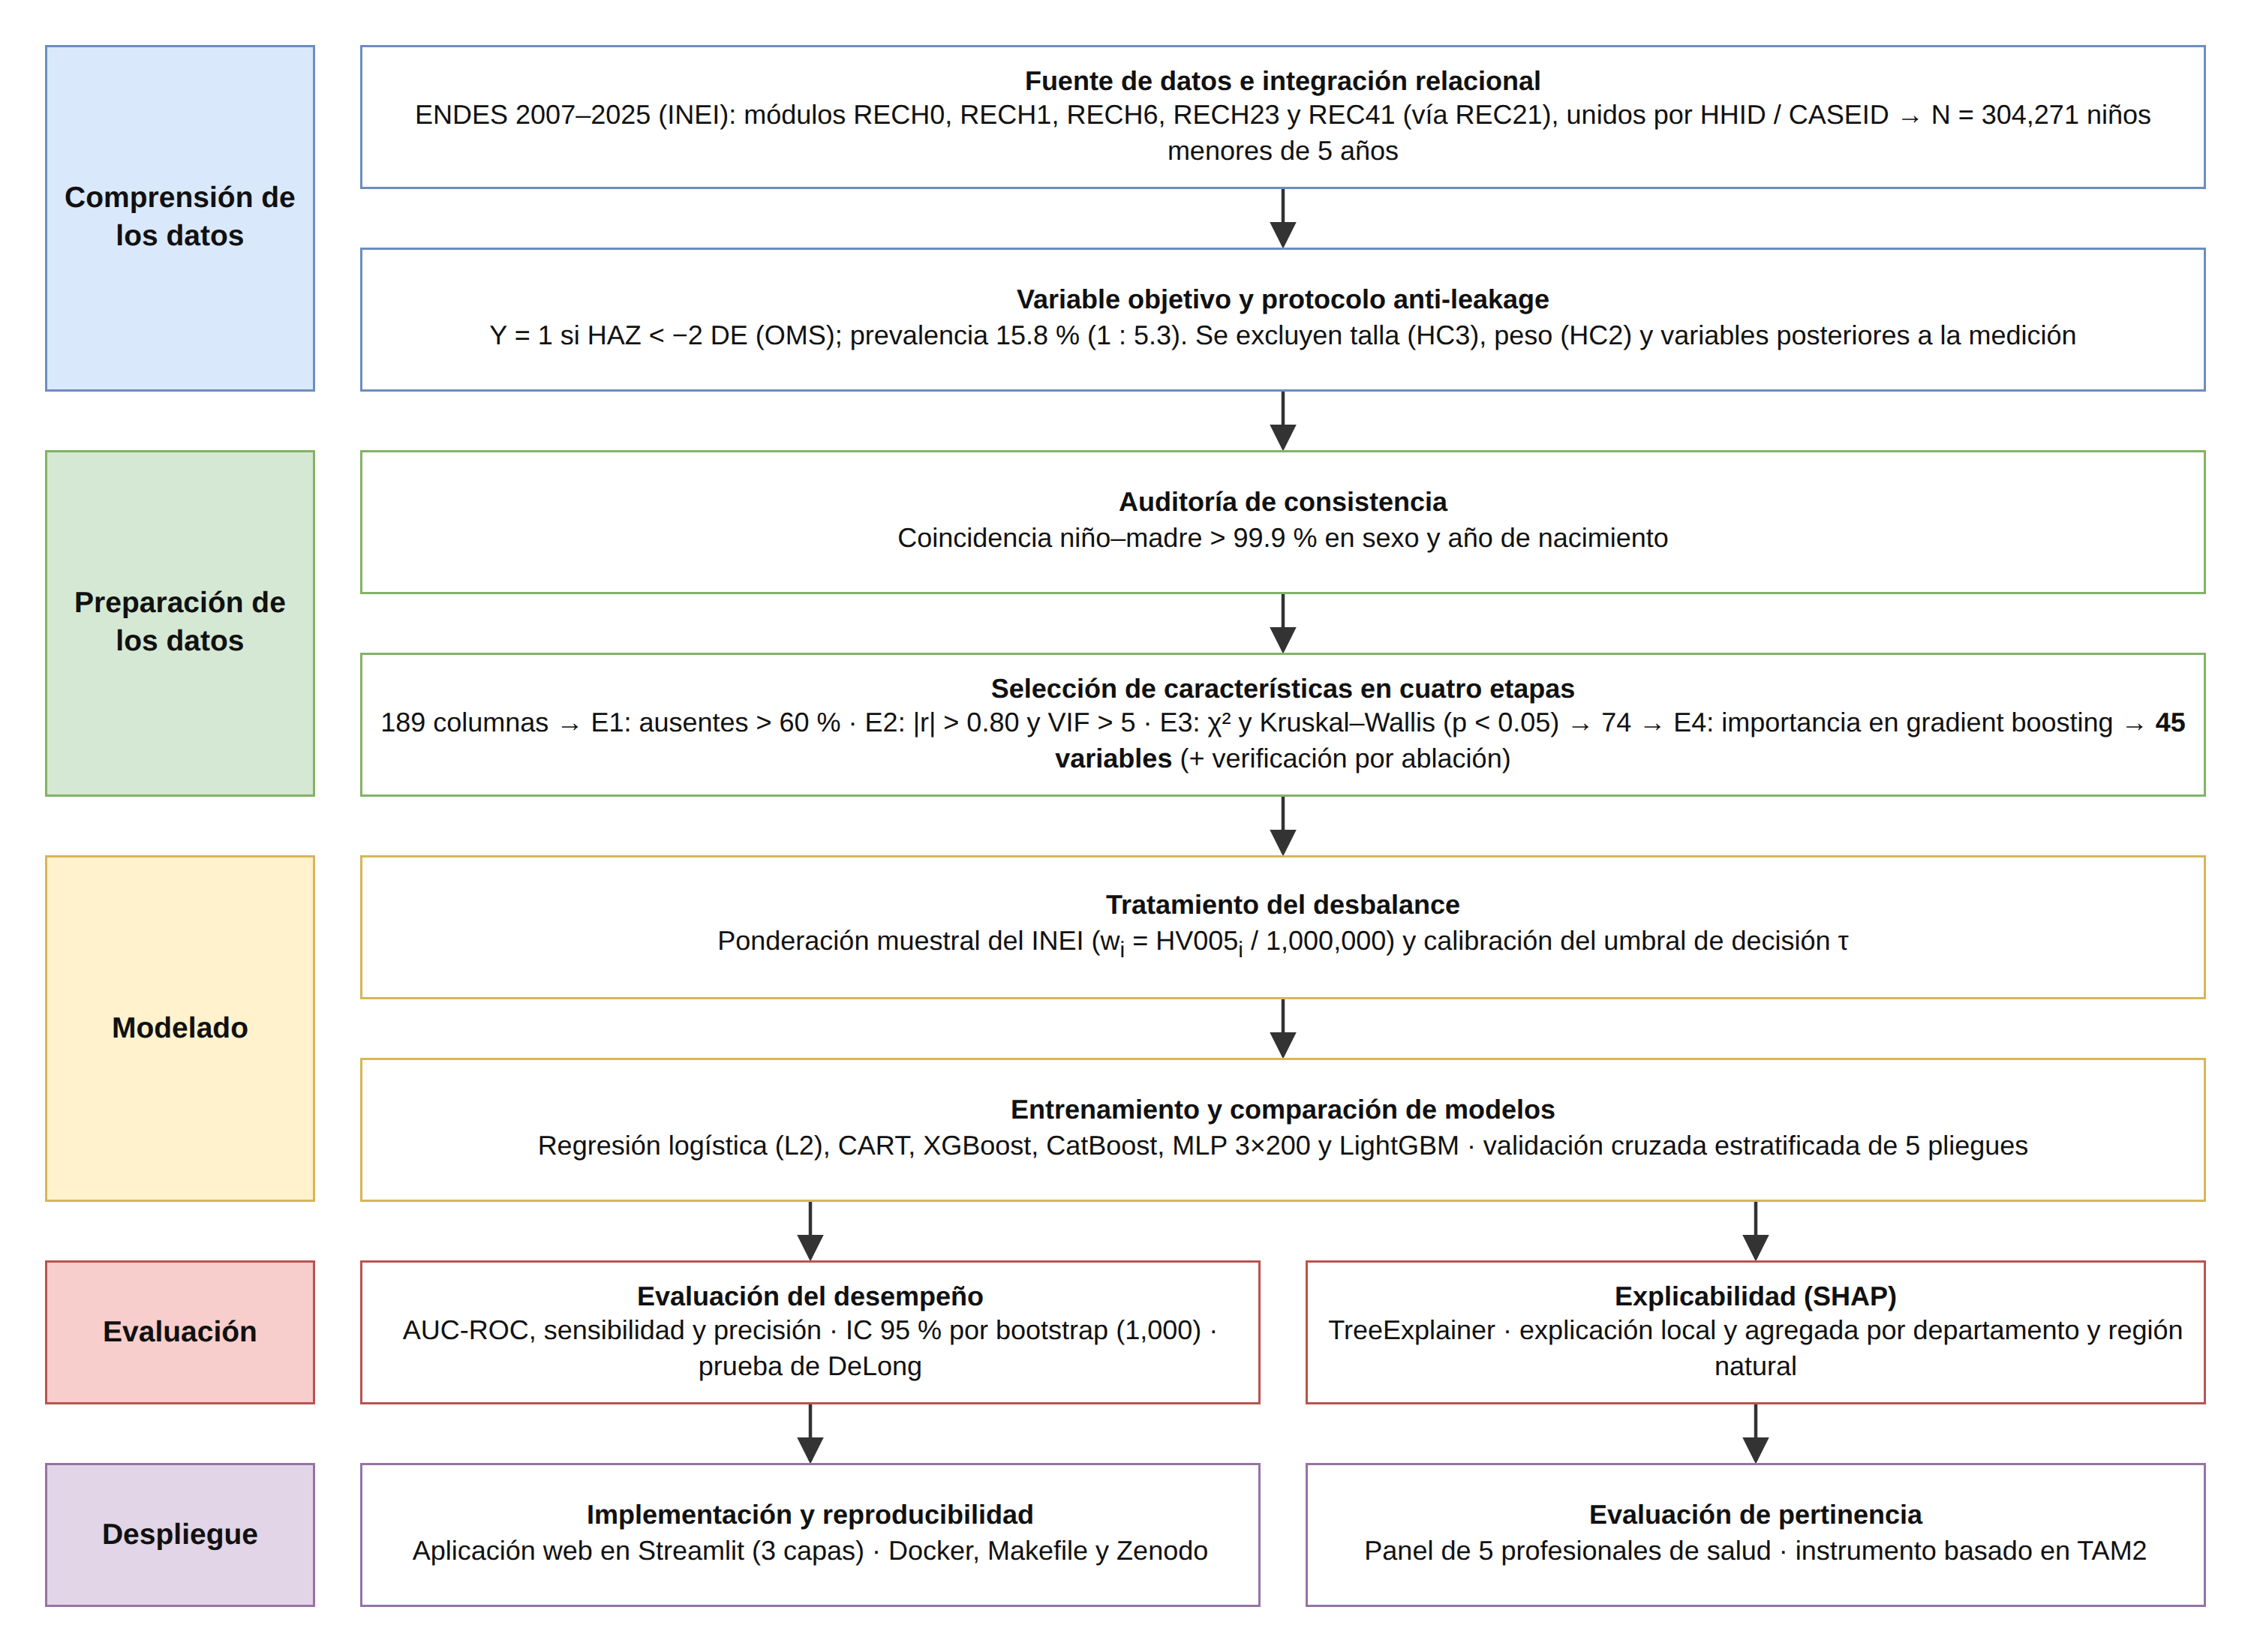
\includegraphics[width=0.98\textwidth]{prism-uploads/Figura1_flujo_metodologico (1).png}
\caption{Flujo metodológico del estudio según las fases de CRISP-DM.}
\label{fig:flujo_metodologico}
\end{figure*}

\subsection{Fuente de datos e integración relacional}

El estudio utilizó los microdatos anuales de la Encuesta Demográfica y de Salud Familiar (ENDES), recolectados y publicados por el Instituto Nacional de Estadística e Informática (INEI) del Perú entre 2007 y 2025. Para estructurar la unidad de análisis, se diseñó un flujo de extracción e integración relacional que vinculó cinco módulos mediante las llaves \texttt{HHID} y \texttt{CASEID}. El módulo RECH0 proveyó los metadatos de la entrevista; RECH1, las características demográficas de los integrantes del hogar; RECH6, los indicadores antropométricos y de salud infantil; RECH23, las condiciones de vivienda y saneamiento, además de la altitud geográfica, relacionada con la concentración de hemoglobina en la población infantil peruana \citep{accinelli2020anemia}; y REC41, la historia obstétrica materna, los controles prenatales y el peso al nacer. Este último se vinculó de forma unívoca con el registro infantil mediante la tabla puente REC21. La integración y la auditoría de consistencia niño--madre presentaron una coincidencia superior al 99.9~\% en sexo y año de nacimiento. La muestra consolidada incluyó 304,271 niños y niñas menores de cinco años con registros antropométricos válidos; la Figura~\ref{fig:integracion_endes} resume la estructura de integración.

\begin{figure*}[t]
\centering
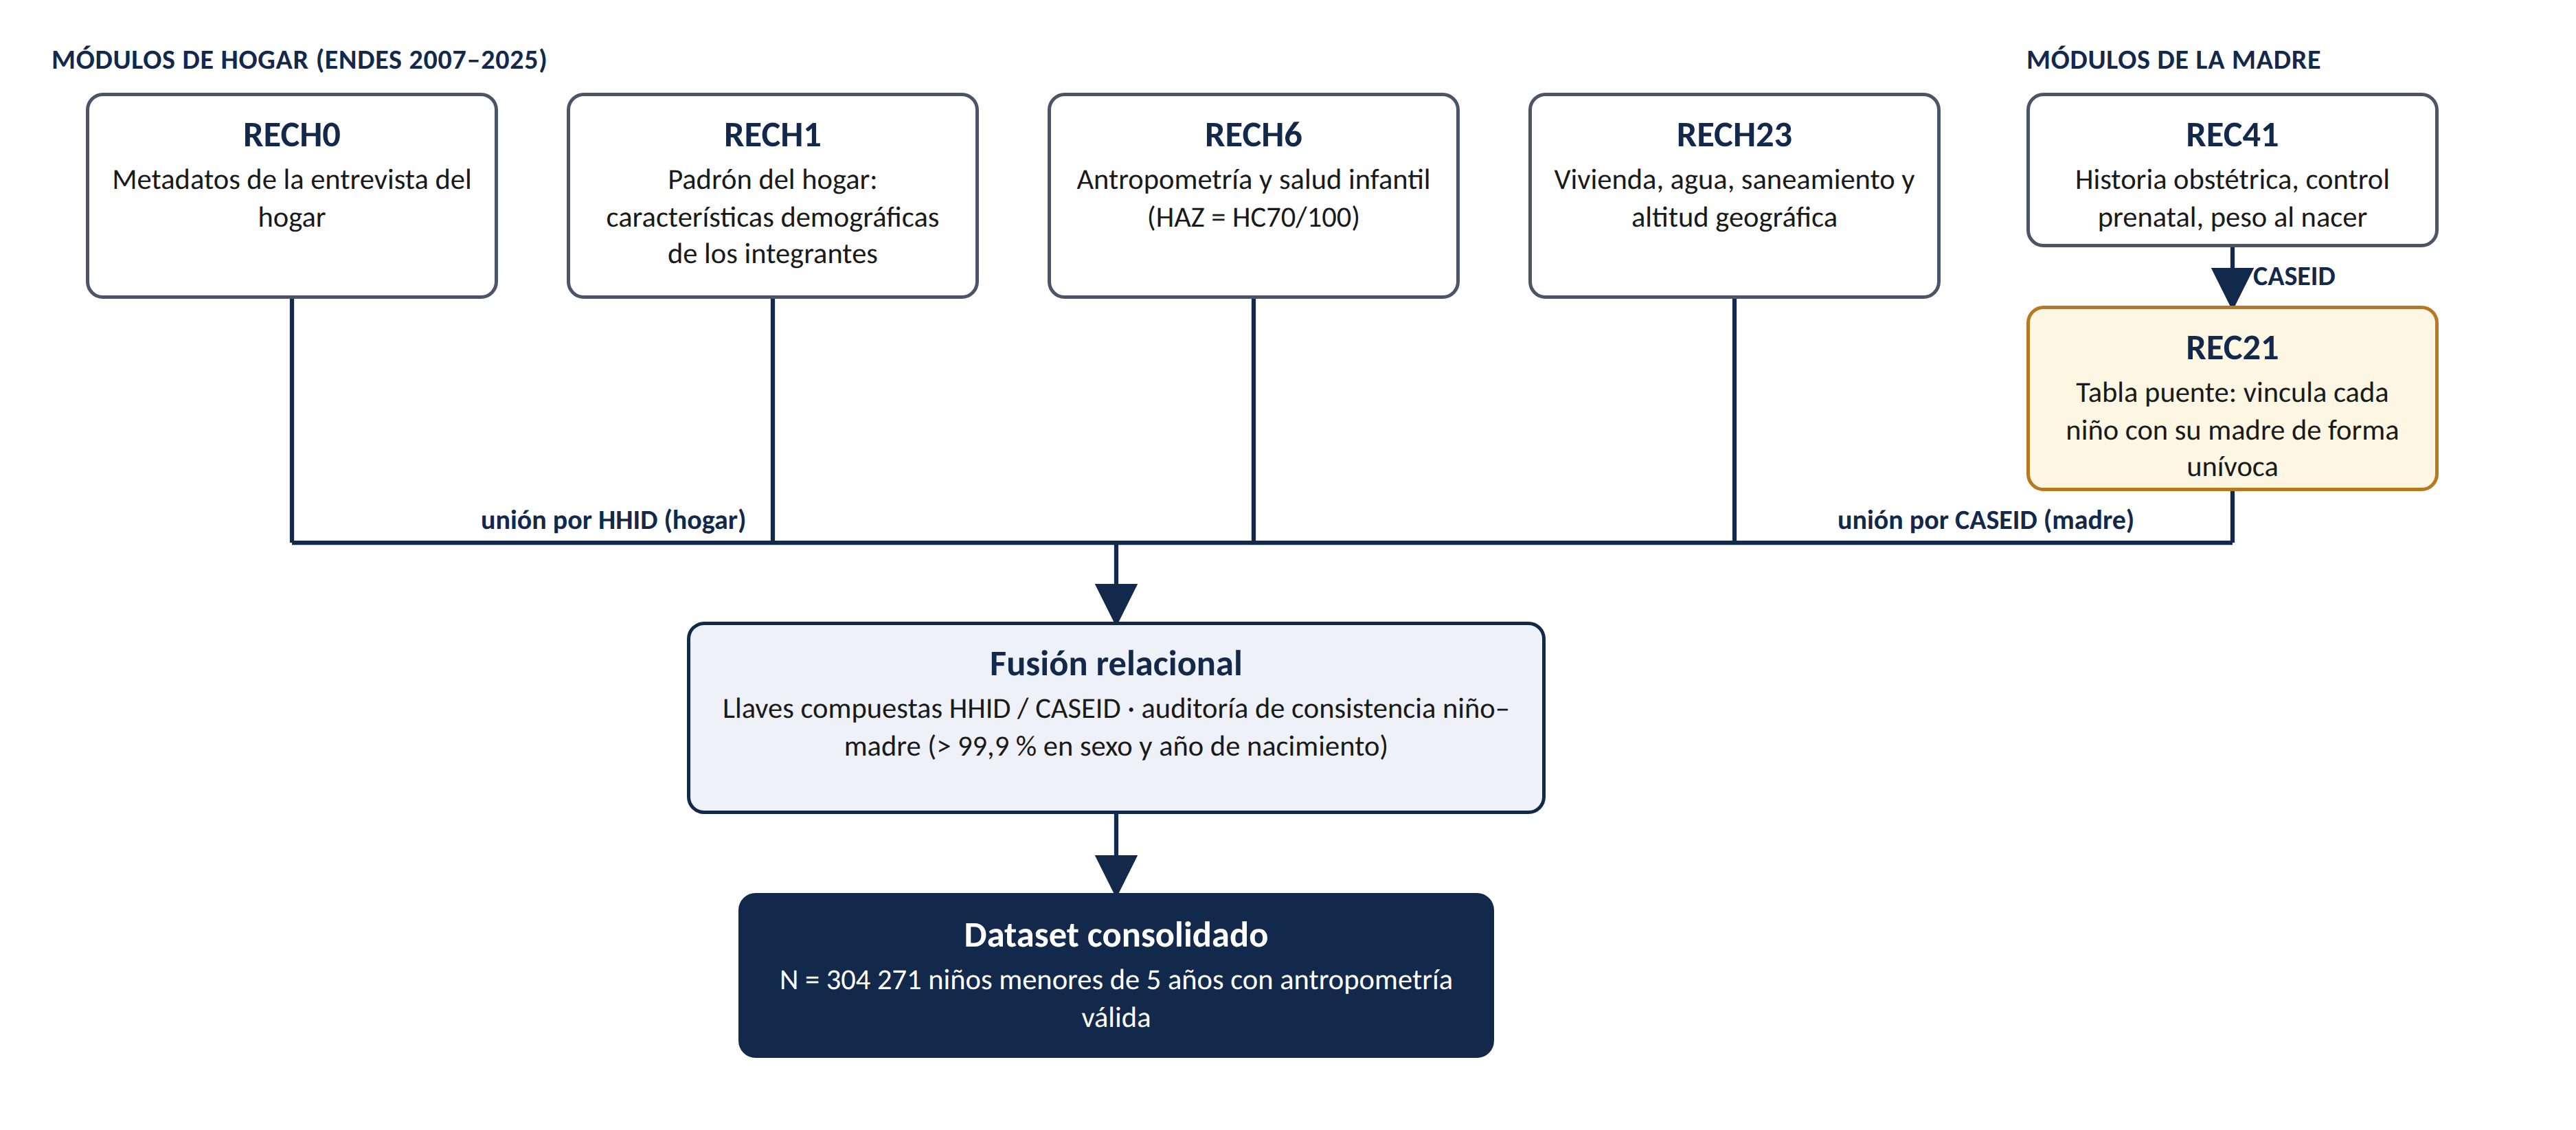
\includegraphics[width=0.98\textwidth]{prism-uploads/Figura2_integracion_ENDES.png}
\caption{Integración relacional de los módulos de la ENDES 2007--2025 mediante las llaves \texttt{HHID} y \texttt{CASEID}.}
\label{fig:integracion_endes}
\end{figure*}

\subsection{Definición de la variable objetivo y protocolo anti-leakage}

La variable dependiente es la desnutrición crónica infantil, categorizada de acuerdo con los estándares internacionales de crecimiento de la Organización Mundial de la Salud, criterio empleado sistemáticamente en el análisis de la desnutrición infantil peruana \citep{sobrino2014peru,santos2021peru}. Se definió como caso positivo ($Y=1$) a todo infante cuyo puntaje Z de talla para la edad ($\mathrm{HAZ}=\mathrm{HC70}/100$) se situó por debajo de menos dos desviaciones estándar respecto de la mediana de referencia, y como caso control ($Y=0$) en caso contrario. La prevalencia global en la serie histórica fue del 15.8~\%, con una razón de desbalance de 1:5.3. Para preservar la validez metodológica y evitar el sobreajuste espurio por fuga de datos (data leakage) \citep{kaufman2011leakage}, se excluyeron de las variables predictoras la talla directa en centímetros (HC3), el peso crudo (HC2) y cualquier intervención terapéutica o diagnóstico clínico registrado después de la medición antropométrica.

\begin{equation}
Y =
\begin{cases}
1, & \text{si } \mathrm{HAZ} < -2.00\text{ DE},\\
0, & \text{si } \mathrm{HAZ} \geq -2.00\text{ DE}.
\end{cases}
\label{eq:variable_objetivo}
\end{equation}

\subsection{Preprocesamiento y selección de características}

Antes de la selección de variables, se armonizaron los códigos de las distintas rondas de la encuesta, se trataron los valores ausentes y se codificaron las variables categóricas para construir un espacio de características comparable entre años. Asimismo, se verificó la consistencia biológica entre los registros del niño y de la madre, descrita en la subsección anterior. El flujo de preparación y selección partió de 189 columnas crudas y se desarrolló en cuatro etapas cuantitativas.

Primero, se descartaron los atributos con más del 60~\% de valores ausentes estructurales históricos. Segundo, se redujo la redundancia dimensional mediante la eliminación de variables colineales, utilizando correlaciones bivariadas de Pearson y Spearman ($r>0.80$) y factores de inflación de varianza ($\mathrm{VIF}>5$). Tercero, se aplicaron pruebas de independencia de chi-cuadrado para variables categóricas y pruebas no paramétricas de Kruskal--Wallis para variables continuas; se retuvieron 74 factores estadísticamente significativos ($p<0.05$). Cuarto, se evaluó la importancia multivariada mediante árboles de decisión potenciados por gradiente y se seleccionaron 45 variables predictoras.

\subsubsection{Verificación de suficiencia del subconjunto seleccionado}

Para descartar que la reducción dimensional hubiese eliminado señal predictiva relevante, se realizó un estudio de ablación sobre las variables excluidas. De las 78 columnas disponibles en el conjunto preprocesado, 33 no formaron parte de las 45 seleccionadas. Estas se ordenaron según su señal marginal respecto de la variable objetivo: para los atributos categóricos se empleó la amplitud entre las tasas de prevalencia máxima y mínima de categorías con al menos 500 observaciones, mientras que para las variables continuas se utilizó el estadístico $2\lvert\mathrm{AUC}-0.5\rvert$.

El procedimiento identificó diez atributos con señal marginal elevada: material predominante de las paredes (HV214), del piso (HV213) y del techo (HV215); fuente de abastecimiento de agua (HV201); departamento de residencia (HV024); concentración de cloro residual en el agua (SH227); combustible utilizado para cocinar (HV226); y tipo de servicio higiénico (HV205), entre otros. Estos atributos conforman el bloque de agua, saneamiento, higiene y condiciones materiales de la vivienda, reconocido como determinante subyacente del retraso del crecimiento lineal \citep{black2013lancet,victora2021lancet} y recuperado entre los predictores principales en estudios basados en datos DHS \citep{bitew2021ethiopia}. Ninguno constituye fuga de información, pues describen condiciones estructurales del hogar observables antes de una visita domiciliaria.

Se contrastaron cuatro configuraciones experimentales manteniendo constantes la partición, la ponderación muestral, la semilla determinista y los hiperparámetros del clasificador. La configuración de referencia reprodujo las cifras del modelo campeón (AUC = 0.8295; Recall = 76.44~\%), lo que verificó la trazabilidad del experimento.

\begin{table*}[t]
\centering
\caption{Estudio de ablación del subconjunto de características.}
\label{tab:ablacion}
\begin{tabular}{lcccc}
\hline
Configuración & Atributos & AUC-ROC & Recall & Precisión \\
\hline
Subconjunto seleccionado & 45 & 0.8295 & 76.44~\% & 36.36~\% \\
Agua, saneamiento y vivienda & 52 & 0.8295 & 76.44~\% & 36.36~\% \\
Atributos territoriales & 48 & 0.8295 & 76.44~\% & 36.36~\% \\
Ampliación conjunta & 55 & 0.8295 & 76.44~\% & 36.36~\% \\
\hline
\end{tabular}
\end{table*}

La incorporación de los diez atributos no produjo mejoras en la capacidad discriminativa: el AUC-ROC, la sensibilidad y la precisión permanecieron invariables hasta la cuarta cifra decimal. El análisis descartó la ausencia de señal, pues un clasificador entrenado únicamente con el bloque de agua, saneamiento y vivienda alcanzó un AUC-ROC de 0.6895, así como la redundancia lineal con el índice de riqueza, cuya varianza explicada por cada atributo candidato se situó entre $\eta^2=0.038$ y $\eta^2=0.098$. El subconjunto de 45 variables ya representa el constructo latente de las condiciones materiales del hogar mediante diecinueve atributos correlacionados, por lo que la exclusión de las variables candidatas constituye una decisión metodológicamente sustentada.

\subsection{Tratamiento del desbalance de clases}

Para reflejar la distribución demográfica del país y corregir el sesgo de sobremuestreo urbano de la encuesta, se incorporó el factor de ponderación muestral del INEI, $w_i=\mathrm{HV005}_i/1{,}000{,}000$, tanto durante el entrenamiento como en el cálculo de las métricas. Además, el umbral de decisión $\tau$ se calibró con un criterio de triaje preventivo que prioriza la cobertura de los casos positivos, en lugar de asumir automáticamente el valor convencional de 0.5.

\subsection{Entrenamiento y comparación de modelos}

Se evaluaron seis algoritmos supervisados: Regresión Logística con regularización L2, Árbol de Decisión CART, XGBoost, CatBoost, Red Neuronal Perceptrón Multicapa (MLP de tres capas ocultas con 200 neuronas cada una) y LightGBM. La comparación utilizó validación cruzada estratificada de cinco pliegues y una semilla determinista (\texttt{random\_state = 42}). LightGBM permite agrupar variables categóricas de alta cardinalidad mediante histogramas, sin recurrir a expansión One-Hot \citep{bentejac2021gradientboosting}. La selección de estos algoritmos, en particular de los ensambles basados en árboles, es coherente con estudios sobre datos DHS que reportan su utilidad para predecir la desnutrición infantil \citep{bitew2021ethiopia,talukder2020bangladesh,chilyabanyama2022zambia}.

\subsection{Estrategia de validación y métricas de evaluación}

La evaluación del desempeño se basó en las probabilidades fuera de pliegue (out-of-fold) de los 304,271 registros, siguiendo las recomendaciones para reportar modelos predictivos en salud \citep{moons2015tripod}. Se calcularon AUC-ROC, sensibilidad, precisión y especificidad con ponderación muestral. La incertidumbre de las estimaciones se cuantificó mediante 1,000 repeticiones de bootstrap no paramétrico y sus intervalos de confianza del 95~\%. La comparación del modelo seleccionado con los modelos de referencia se efectuó con la prueba de DeLong para curvas ROC correlacionadas. Como dicha prueba se basa en rangos y no admite ponderación muestral, se aplicó sobre la muestra sin expandir, utilizando los mismos individuos para todos los modelos.

\subsection{Explicabilidad algorítmica con valores SHAP}

Para aportar transparencia al sistema, se aplicó la teoría de juegos cooperativos mediante el algoritmo TreeExplainer del framework SHAP (SHapley Additive exPlanations) \citep{lundberg2017shap}. Este enfoque descompone la probabilidad predicha en la suma del valor base poblacional y las contribuciones marginales de cada una de las 45 variables predictoras. En el nivel local, el sistema separa la predicción individual en factores de riesgo y condiciones protectoras. En los niveles global y territorial, los valores SHAP se agregaron sobre una muestra representativa de 10,000 registros para construir mapas de riesgo y perfiles de determinantes diferenciados para los 25 departamentos y las tres regiones naturales del país.

\begin{equation}
f(x)=\phi_0+\sum_{j=1}^{M}\phi_j(x).
\label{eq:shap}
\end{equation}

\subsection{Implementación, reproducibilidad y evaluación de pertinencia}

La solución se implementó como una aplicación web interactiva en Streamlit, organizada en tres capas (Figura~\ref{fig:arquitectura}). La capa de presentación integra la visualización coroplética departamental basada en geometrías GeoJSON, la evaluación de un niño con la explicación de su puntaje y la evaluación de un grupo de niños a partir de un archivo CSV o Excel, que devuelve una lista ordenada por riesgo. La capa lógica reúne el motor de inferencia LightGBM, el selector del umbral de prioridad según la cobertura elegida y el cálculo de la contribución de cada variable mediante valores SHAP en tiempo de ejecución. La capa de datos contiene el modelo serializado y sus metadatos, la curva cobertura--umbral, los valores SHAP agregados por departamento y las geometrías departamentales; el conjunto maestro en formato Parquet se utiliza únicamente en el flujo de entrenamiento.

\begin{figure*}[t]
\centering
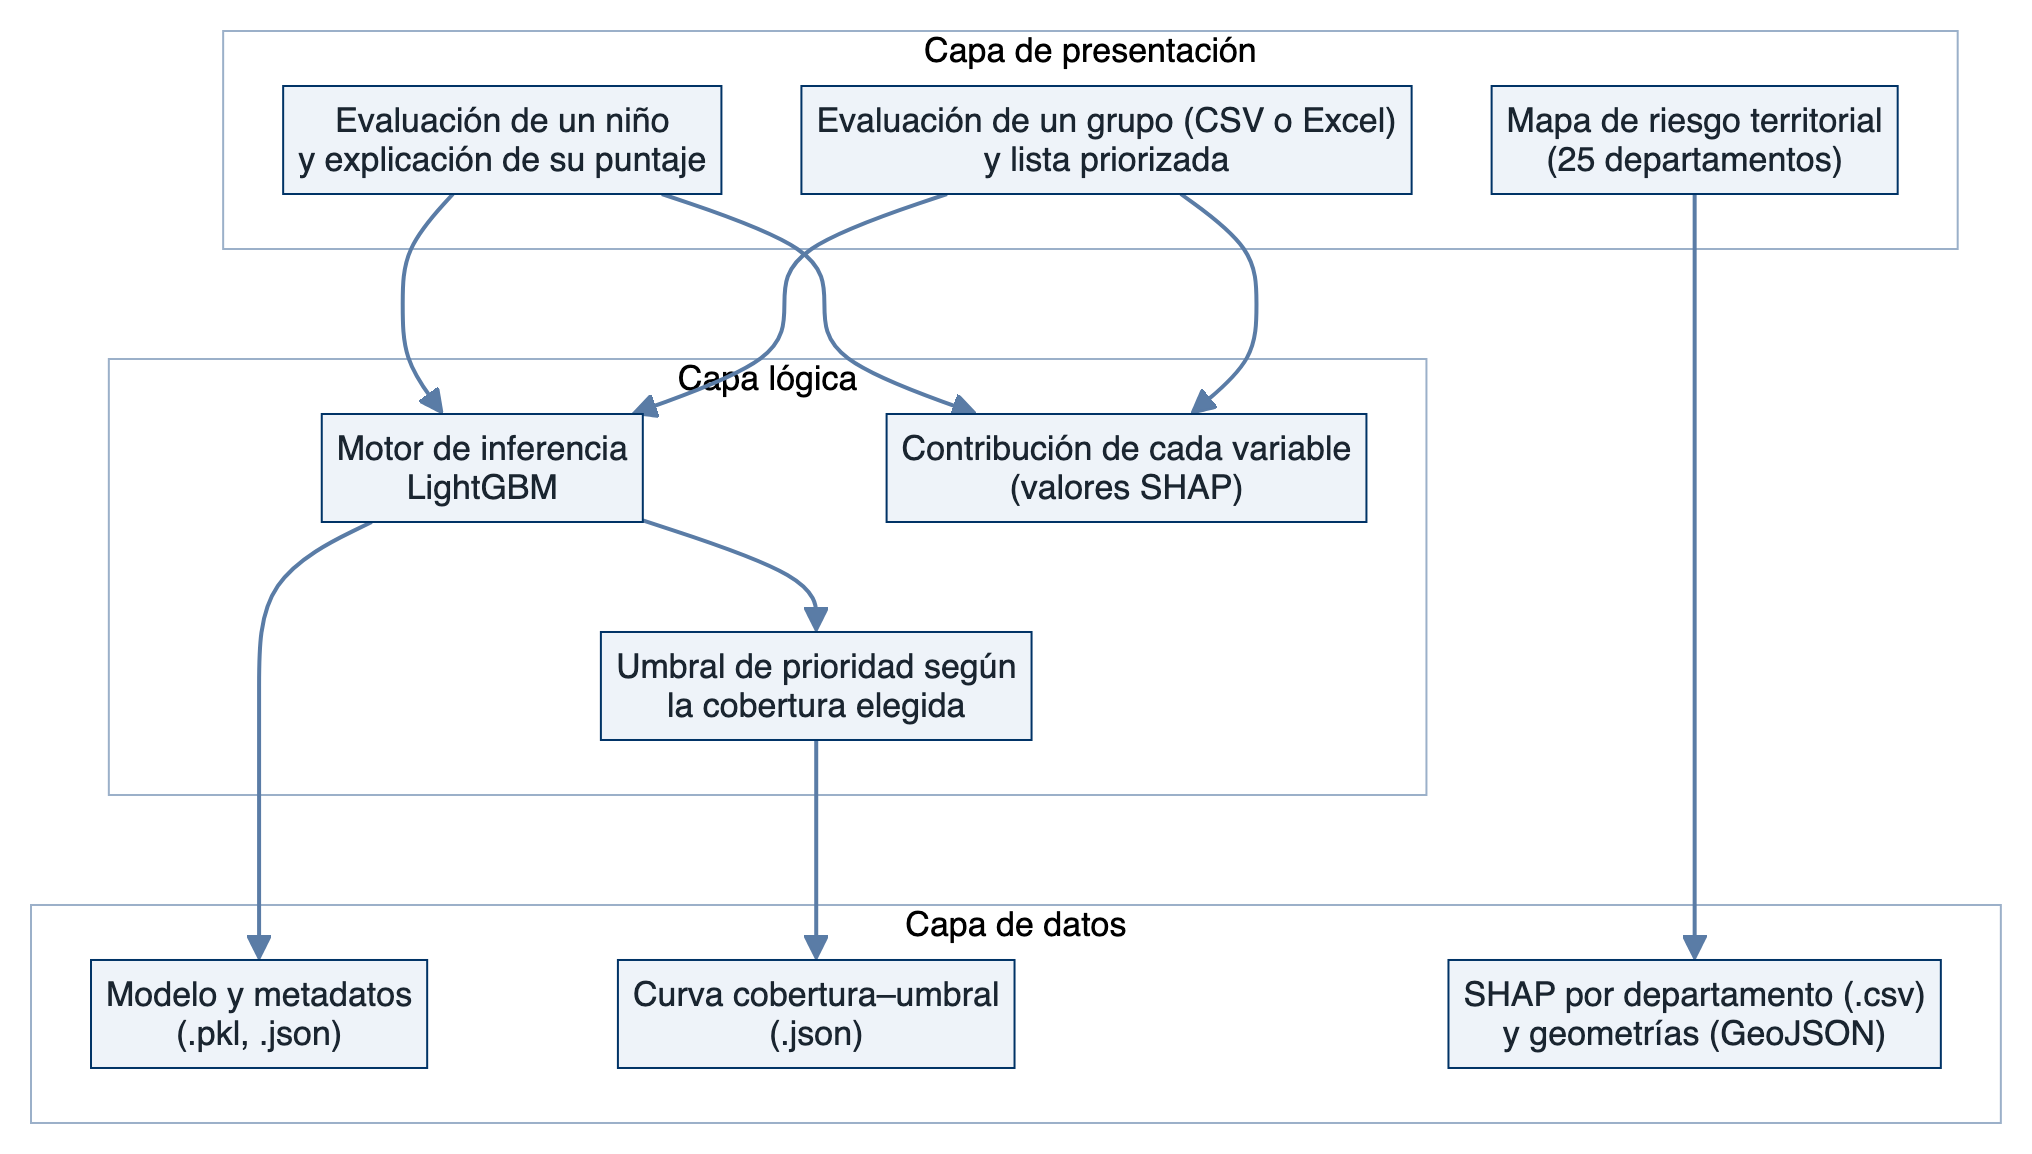
\includegraphics[width=0.85\textwidth]{prism-uploads/Figura3_arquitectura_software.png}
\caption{Arquitectura de la solución en tres capas: presentación, lógica y datos.}
\label{fig:arquitectura}
\end{figure*}

La reproducibilidad se abordó de acuerdo con los principios FAIR mediante la modularización del código en el paquete Python \texttt{mnp/}, el aislamiento del entorno con Docker (\texttt{python:3.12-slim}), la automatización del flujo con Makefile y la publicación del conjunto de datos maestro y del modelo serializado en Zenodo.

La pertinencia se evaluó mediante un panel de cuatro profesionales sanitarios: tres nutricionistas y un enfermero, todos con al menos diez años de experiencia asistencial y grado de maestría. La evaluación se apoyó en el Modelo de Aceptación Tecnológica \citep{davis1989tam} y en su extensión TAM2 \citep{venkatesh2000tam2}; la utilidad percibida fue el criterio central, por el propósito del sistema de aportar información accionable para priorizar la atención sanitaria.

\subsubsection{Instrumento de evaluación de la pertinencia}

La selección del modelo de aceptación siguió el marco de decisión de \citet{britto2026framework}, que compara TAM, TAM2, TAM3, UTAUT y UTAUT2 según el contexto, el régimen de uso, la etapa de adopción, el foco explicativo y la granularidad. Se eligió TAM2 por tratarse de una evaluación organizacional de aceptación inicial con un panel reducido. De TAM3 \citep{venkatesh2008tam3} se incorporó únicamente la percepción de control externo, para determinar si los datos requeridos por el sistema están disponibles en la práctica asistencial; se omitieron los constructos de imagen y voluntariedad, que no corresponden a especialistas que evalúan la herramienta sin obligación de adoptarla.

Los ítems se adaptaron al contexto sanitario a partir de las escalas de \citet{venkatesh2000tam2}, conservando en cada constructo enunciados con contenido diferenciado y al menos dos ítems. La Tabla~\ref{tab:constructos_tam} detalla los constructos, su modelo de origen y el número de ítems de cada uno. El instrumento consta de 19 afirmaciones en escala Likert de cinco puntos, una valoración global de 1 a 10 y cuatro preguntas abiertas. El ítem K2 consulta específicamente la disponibilidad del dato de hemoglobina, la única variable predictora que requiere un procedimiento sobre el menor. Las respuestas se resumen mediante la mediana y el rango intercuartílico por constructo y el porcentaje de acuerdo por ítem; se considera favorable una mediana igual o superior a 4.

\begin{table*}[t]
\centering
\caption{Constructos del instrumento de evaluación de la pertinencia, modelo de origen e ítems.}
\label{tab:constructos_tam}
\begin{tabular}{lccc}
\hline
Constructo & Modelo de origen & Ítems en la fuente & Ítems del instrumento \\
\hline
Relevancia para el trabajo & TAM2 & 2 & 2 (R1--R2) \\
Calidad del resultado & TAM2 & 2 & 2 (C1--C2) \\
Demostrabilidad del resultado & TAM2 & 4 & 2 (D1--D2) \\
Norma subjetiva & TAM2 & 2 & 2 (S1--S2) \\
Utilidad percibida & TAM & 4 & 3 (U1--U3) \\
Facilidad de uso percibida & TAM & 4 & 3 (F1--F3) \\
Intención de uso & TAM & 2 & 2 (I1--I2) \\
Percepción de control externo & TAM3 & --- & 3 (K1--K3) \\
\hline
\end{tabular}
\end{table*}

\FloatBarrier
\section{Resultados}
\label{resultados}

\FloatBarrier
\subsection{Evolución de la desnutrición crónica, 2007--2025}

La prevalencia ponderada de desnutrición crónica en menores de cinco años descendió de 29.2~\% en 2007 a 13.0~\% en 2017 y, desde 2018, se mantiene entre 11.3~\% y 12.4~\%, con 12.0~\% en 2025 (Figura~\ref{fig:tendencia}). La brecha entre áreas persiste: en 2025 la prevalencia fue de 21.5~\% en el área rural y de 7.9~\% en la urbana.

\begin{figure*}[!t]
\centering
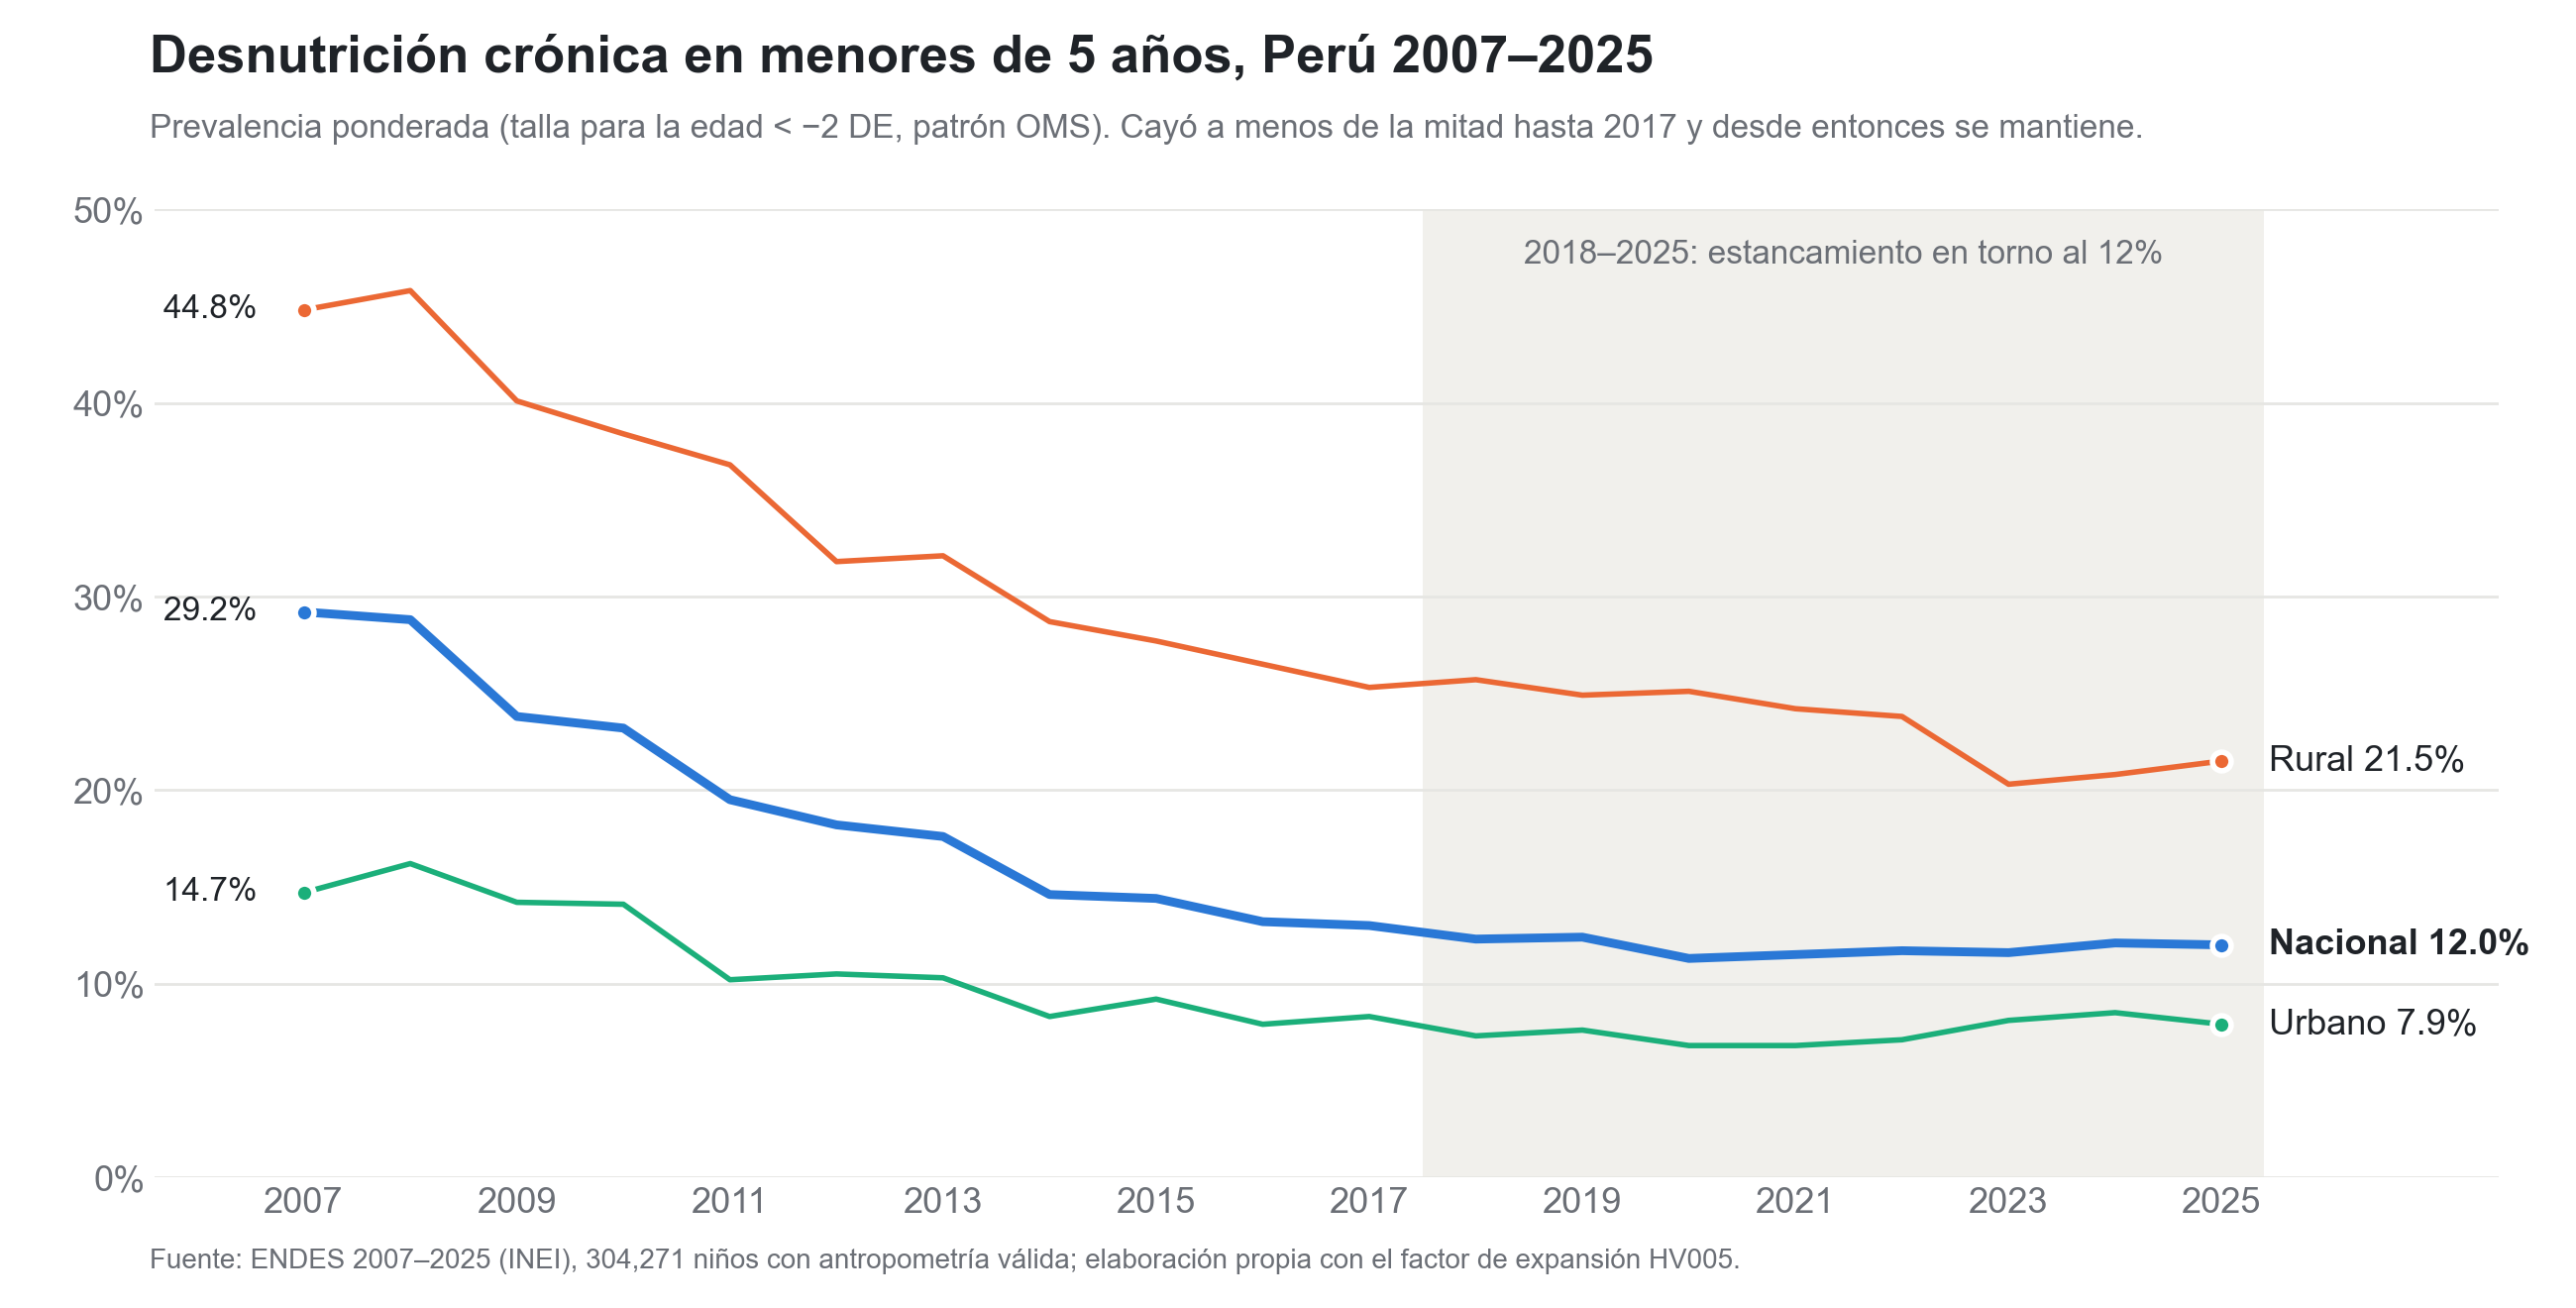
\includegraphics[width=0.8\textwidth]{prism-uploads/Figura4_tendencia_prevalencia.png}
\caption{Prevalencia ponderada de desnutrición crónica en menores de cinco años en el Perú, 2007--2025, a nivel nacional y por área de residencia (talla para la edad menor de $-2$ DE según el patrón OMS; factor de expansión HV005).}
\label{fig:tendencia}
\end{figure*}

\FloatBarrier
\subsection{Comparación de modelos}

Con las probabilidades fuera de pliegue sin ponderación muestral (Tabla~\ref{tab:modelos} y Figuras~\ref{fig:roc}, \ref{fig:pr} y \ref{fig:confusion}), LightGBM alcanzó el mayor AUC-ROC (0.8230), seguido de CatBoost (0.8210) y de la red neuronal (0.8144); la regresión logística, XGBoost y el árbol de decisión se ubicaron entre 0.7696 y 0.7894. CatBoost obtuvo un AUC-PR ligeramente superior (0.5014 frente a 0.4894), pero con el umbral de 0.5 detectó solo el 28.2~\% de los casos, y la red neuronal el 24.2~\%, frente al 75.3~\% de LightGBM. Por su discriminación y su sensibilidad con el umbral de referencia se seleccionó LightGBM. Con ponderación muestral, su AUC-ROC es de 0.8295.

\begin{table*}[!t]
\centering
\caption{Desempeño de los seis algoritmos con las probabilidades fuera de pliegue, sin ponderación muestral (umbral de 0.5).}
\label{tab:modelos}
\begin{tabular}{lcccc}
\hline
Modelo & AUC-ROC & AUC-PR & Sensibilidad & Especificidad \\
\hline
Regresión logística & 0.7894 & 0.4158 & 70.7~\% & 72.9~\% \\
LightGBM & 0.8230 & 0.4894 & 75.3~\% & 73.8~\% \\
XGBoost & 0.7847 & 0.4129 & 74.9~\% & 69.4~\% \\
CatBoost & 0.8210 & 0.5014 & 28.2~\% & 96.4~\% \\
Árbol de decisión & 0.7696 & 0.3840 & 70.4~\% & 71.1~\% \\
Red neuronal & 0.8144 & 0.4798 & 24.2~\% & 96.9~\% \\
\hline
\end{tabular}
\end{table*}

\begin{figure*}[!t]
\centering
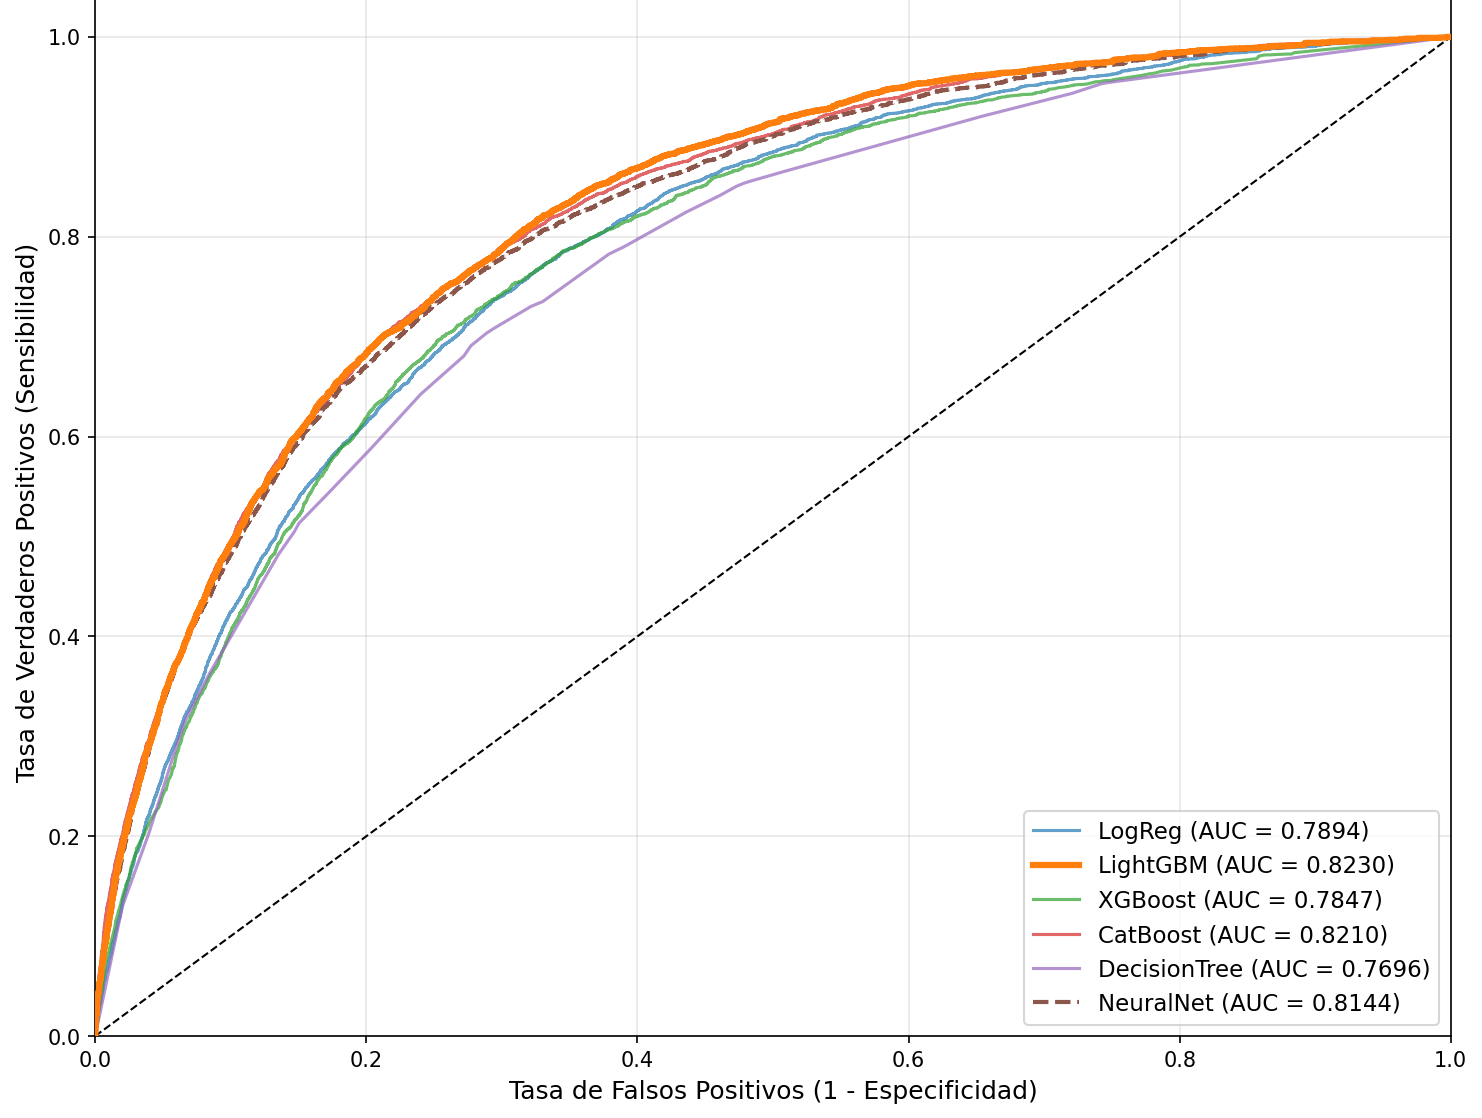
\includegraphics[width=0.6\textwidth]{prism-uploads/Figura5_curvas_roc.png}
\caption{Curvas ROC de los seis algoritmos con las probabilidades fuera de pliegue, sin ponderación muestral.}
\label{fig:roc}
\end{figure*}

\begin{figure*}[!t]
\centering
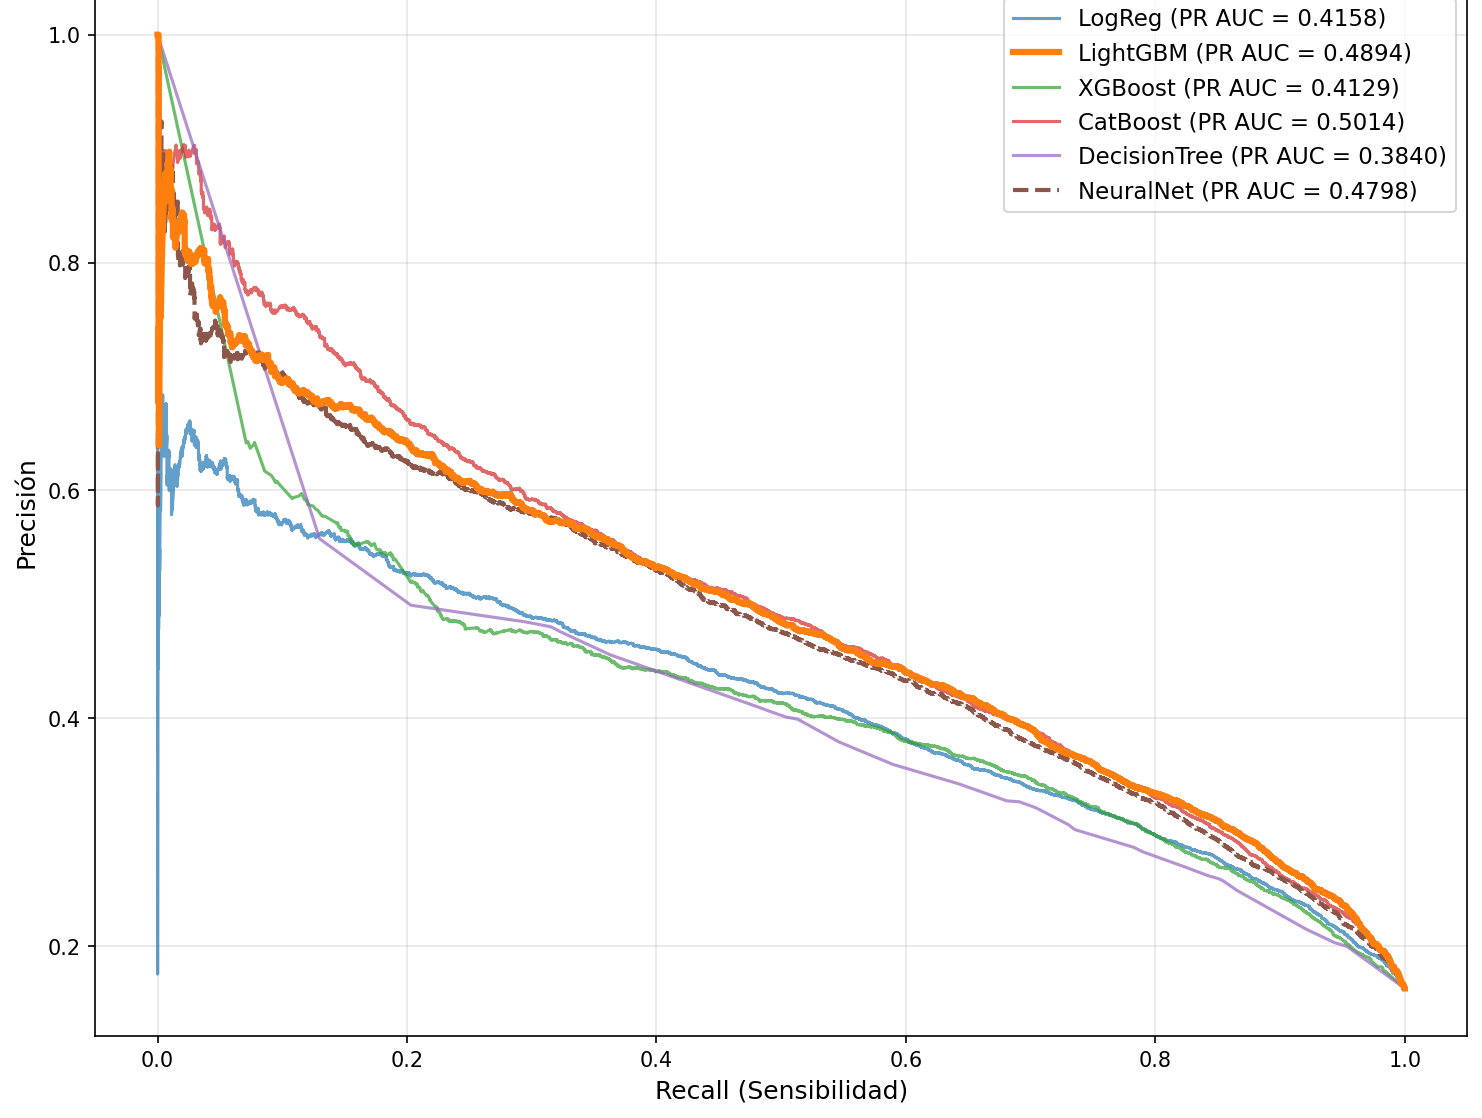
\includegraphics[width=0.6\textwidth]{prism-uploads/Figura6_curvas_precision_recall.png}
\caption{Curvas de precisión--sensibilidad de los seis algoritmos con las probabilidades fuera de pliegue, sin ponderación muestral.}
\label{fig:pr}
\end{figure*}

\begin{figure*}[!t]
\centering
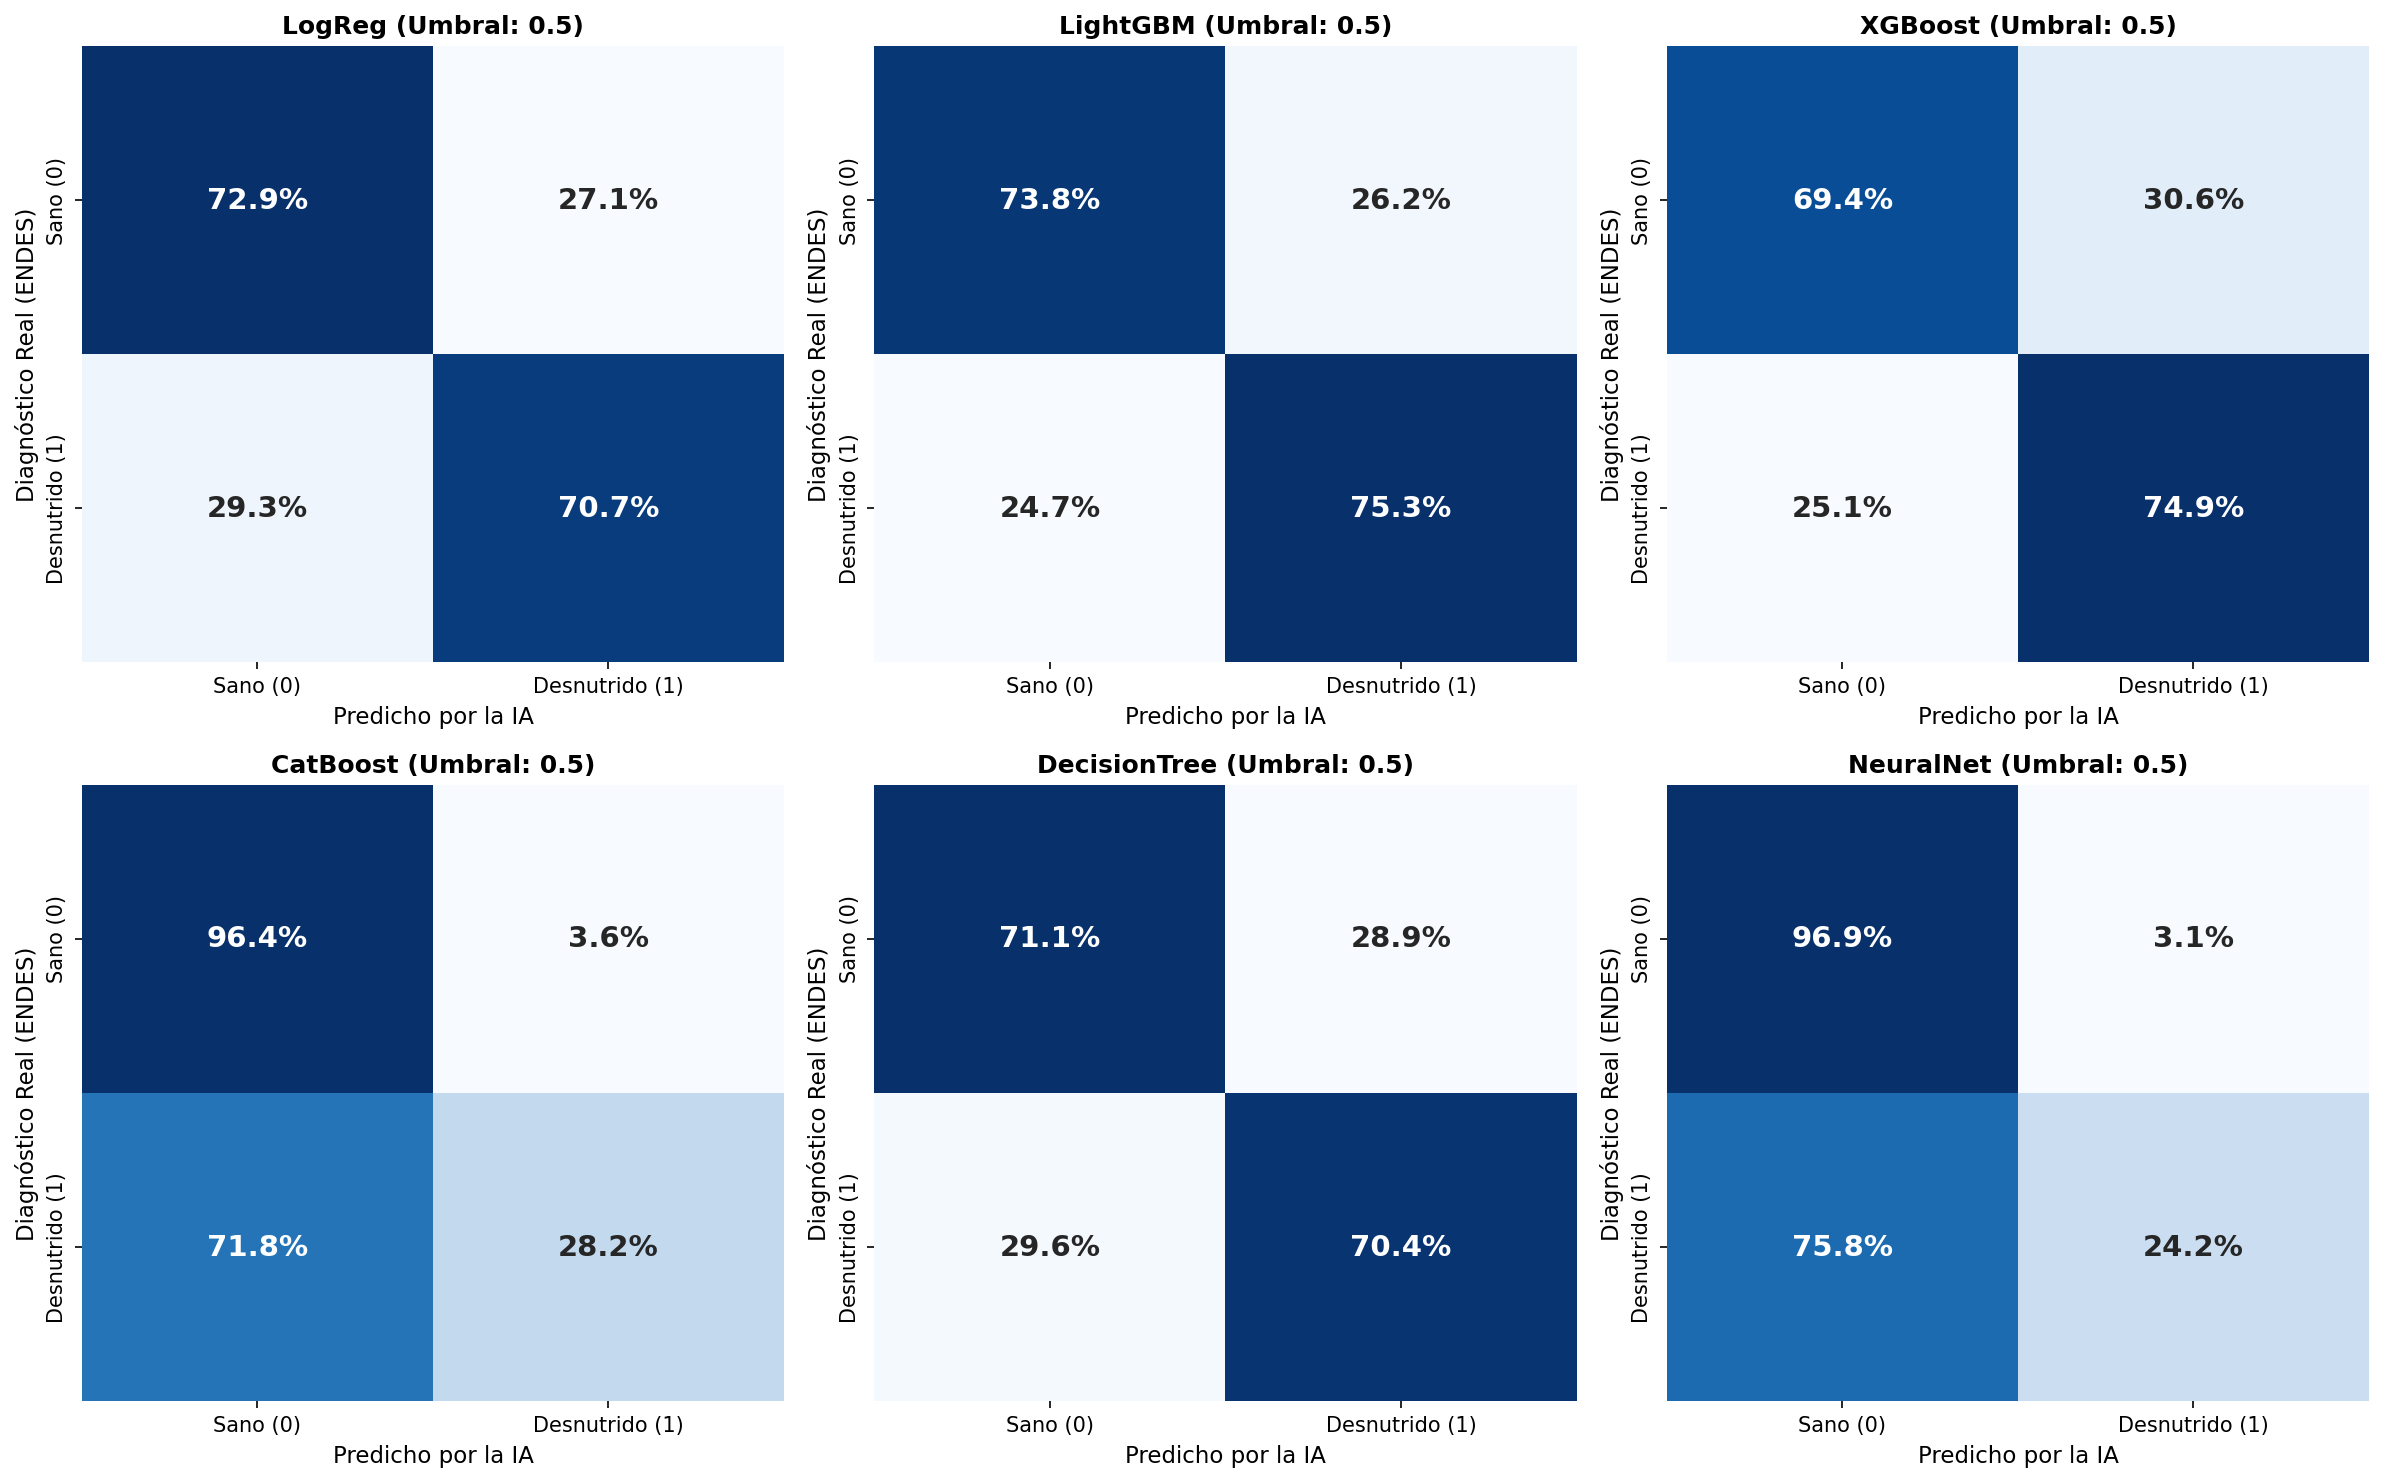
\includegraphics[width=0.8\textwidth]{prism-uploads/Figura7_matrices_confusion.png}
\caption{Matrices de confusión normalizadas por clase real con el umbral de 0.5, sin ponderación muestral.}
\label{fig:confusion}
\end{figure*}

\FloatBarrier
\subsection{Confiabilidad estadística del modelo seleccionado}

Con ponderación muestral, el modelo seleccionado alcanzó un AUC-ROC de 0.8294 (IC 95~\%: 0.8267--0.8324), una sensibilidad de 76.43~\% y una precisión de 36.36~\% con el umbral de 0.5 (Tabla~\ref{tab:bootstrap}). Con el umbral de 0.45, utilizado en la aplicación, la sensibilidad asciende a 80.46~\% y la precisión desciende a 34.04~\%. La prueba de DeLong confirmó la superioridad de LightGBM frente a XGBoost ($z=62.32$) y a la regresión logística ($z=61.48$), con $p<10^{-300}$ en ambos casos y AUC sin ponderar de 0.8193, 0.7775 y 0.7767, respectivamente. Al excluir la hemoglobina, único predictor que exige un procedimiento sobre el niño, el AUC-ROC disminuyó de 0.8294 a 0.8281 (diferencia de $-0.0014$; IC 95~\%: $-0.0019$ a $-0.0009$) y la sensibilidad de 76.43~\% a 76.30~\%.

\begin{table}[!t]
\centering
\caption{Métricas del modelo seleccionado con ponderación muestral e intervalos de confianza de 95~\% por bootstrap (1,000 repeticiones; umbral de 0.5).}
\label{tab:bootstrap}
\begin{tabular}{lcc}
\hline
Métrica & Estimación & IC 95~\% \\
\hline
AUC-ROC & 0.8294 & 0.8267--0.8324 \\
Sensibilidad & 76.43~\% & 75.88--76.98~\% \\
Precisión & 36.36~\% & 35.94--36.71~\% \\
F1 & 49.28~\% & 48.85--49.66~\% \\
\hline
\end{tabular}
\end{table}

\FloatBarrier
\subsection{Explicabilidad}

La importancia global de las variables se concentra en pocos factores (Figura~\ref{fig:shap_global}): la pobreza del hogar (0.42), el peso al nacer (0.41), la altitud de residencia (0.26) y el tamaño al nacer (0.25) destacan claramente, y las diez variables principales acumulan el 68.0~\% de la importancia total. Estos valores describen asociaciones aprendidas de la encuesta y no relaciones causales. El peso de cada factor varía entre territorios (Figura~\ref{fig:mapa_factores}): en Puno destacan la altitud, la pobreza del hogar y el bajo peso al nacer, mientras que en Huancavelica destacan el bajo peso al nacer, el intervalo entre partos y la edad del jefe del hogar.

\begin{figure}[!t]
\centering
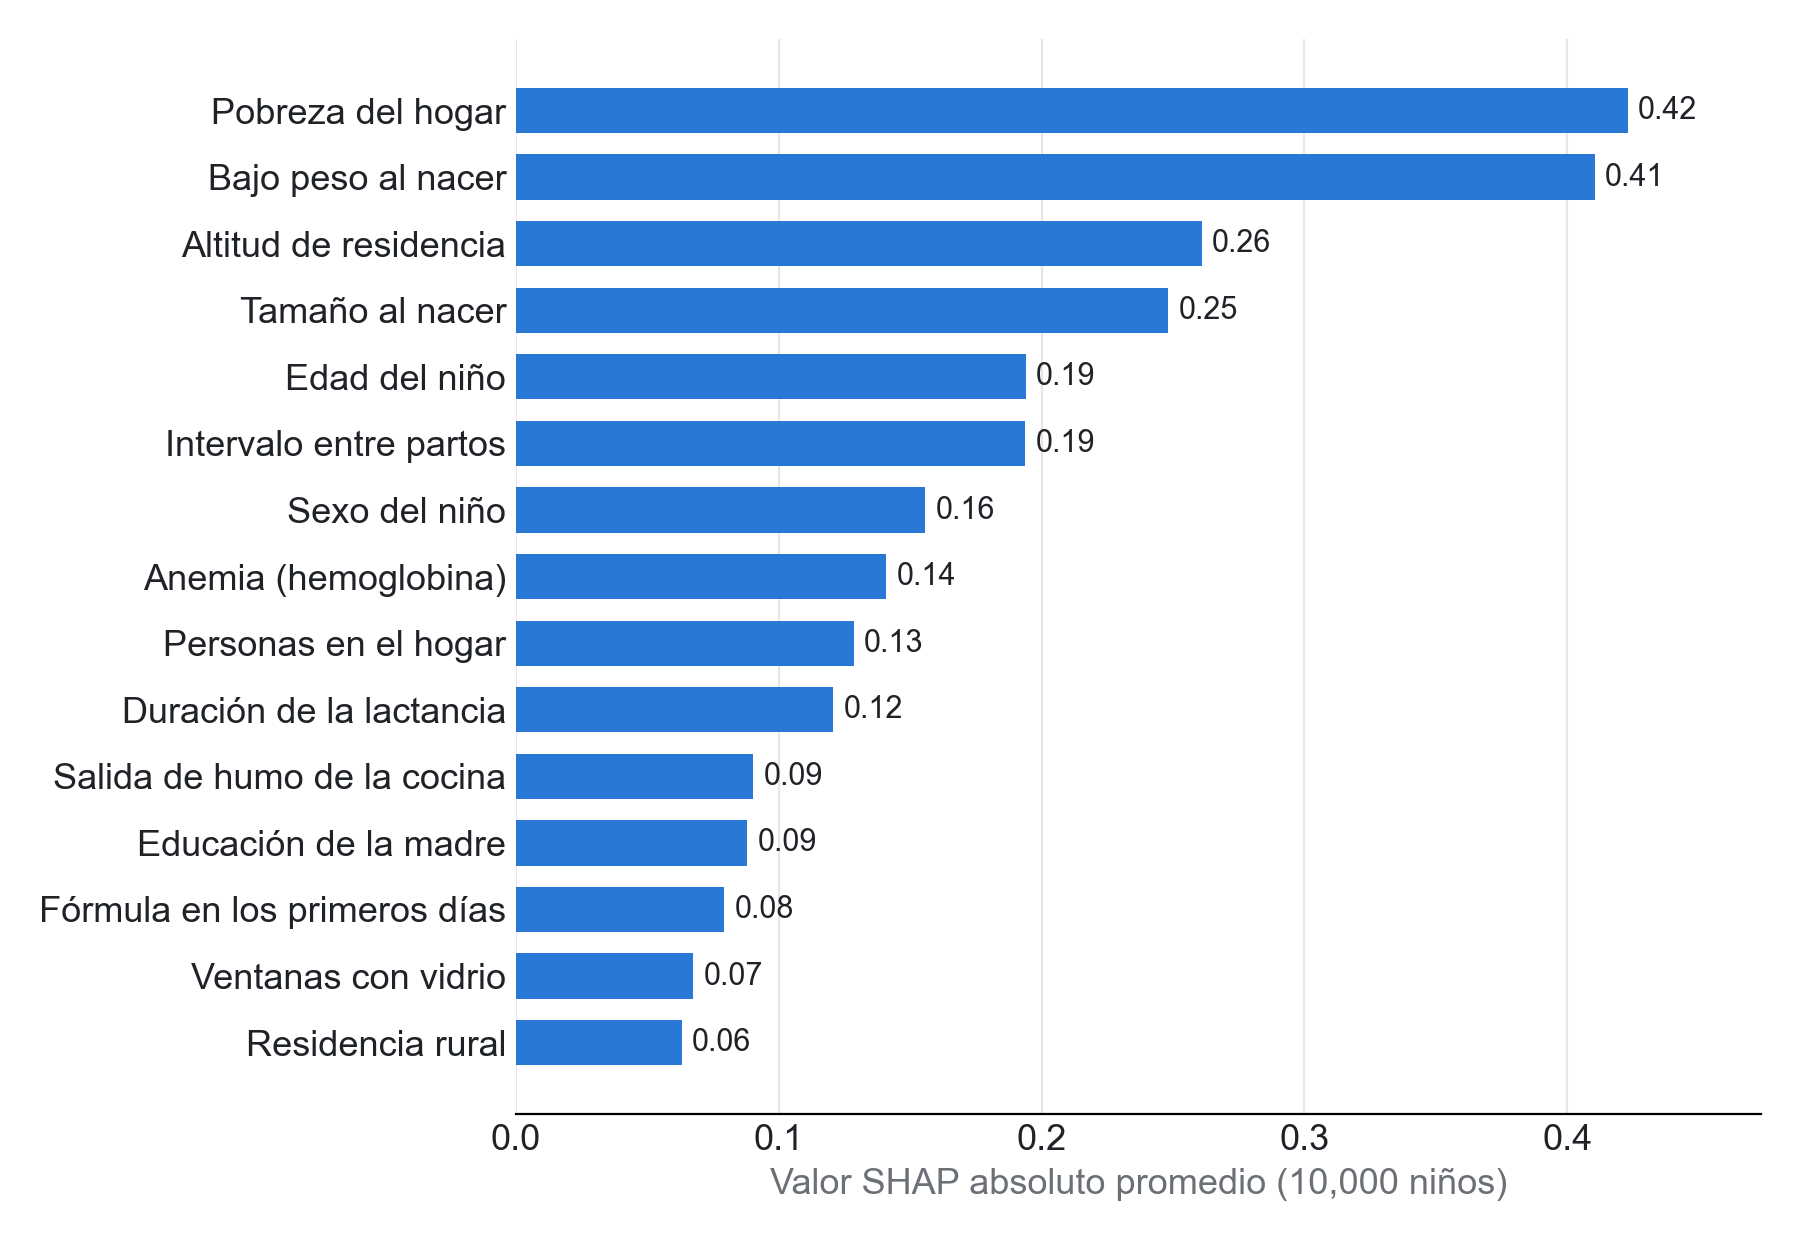
\includegraphics[width=\columnwidth]{prism-uploads/Figura8_importancia_global_shap.png}
\caption{Importancia global de las 15 variables con mayor valor SHAP absoluto promedio del modelo seleccionado, sobre una muestra aleatoria de 10,000 niños.}
\label{fig:shap_global}
\end{figure}

\begin{figure*}[!t]
\centering
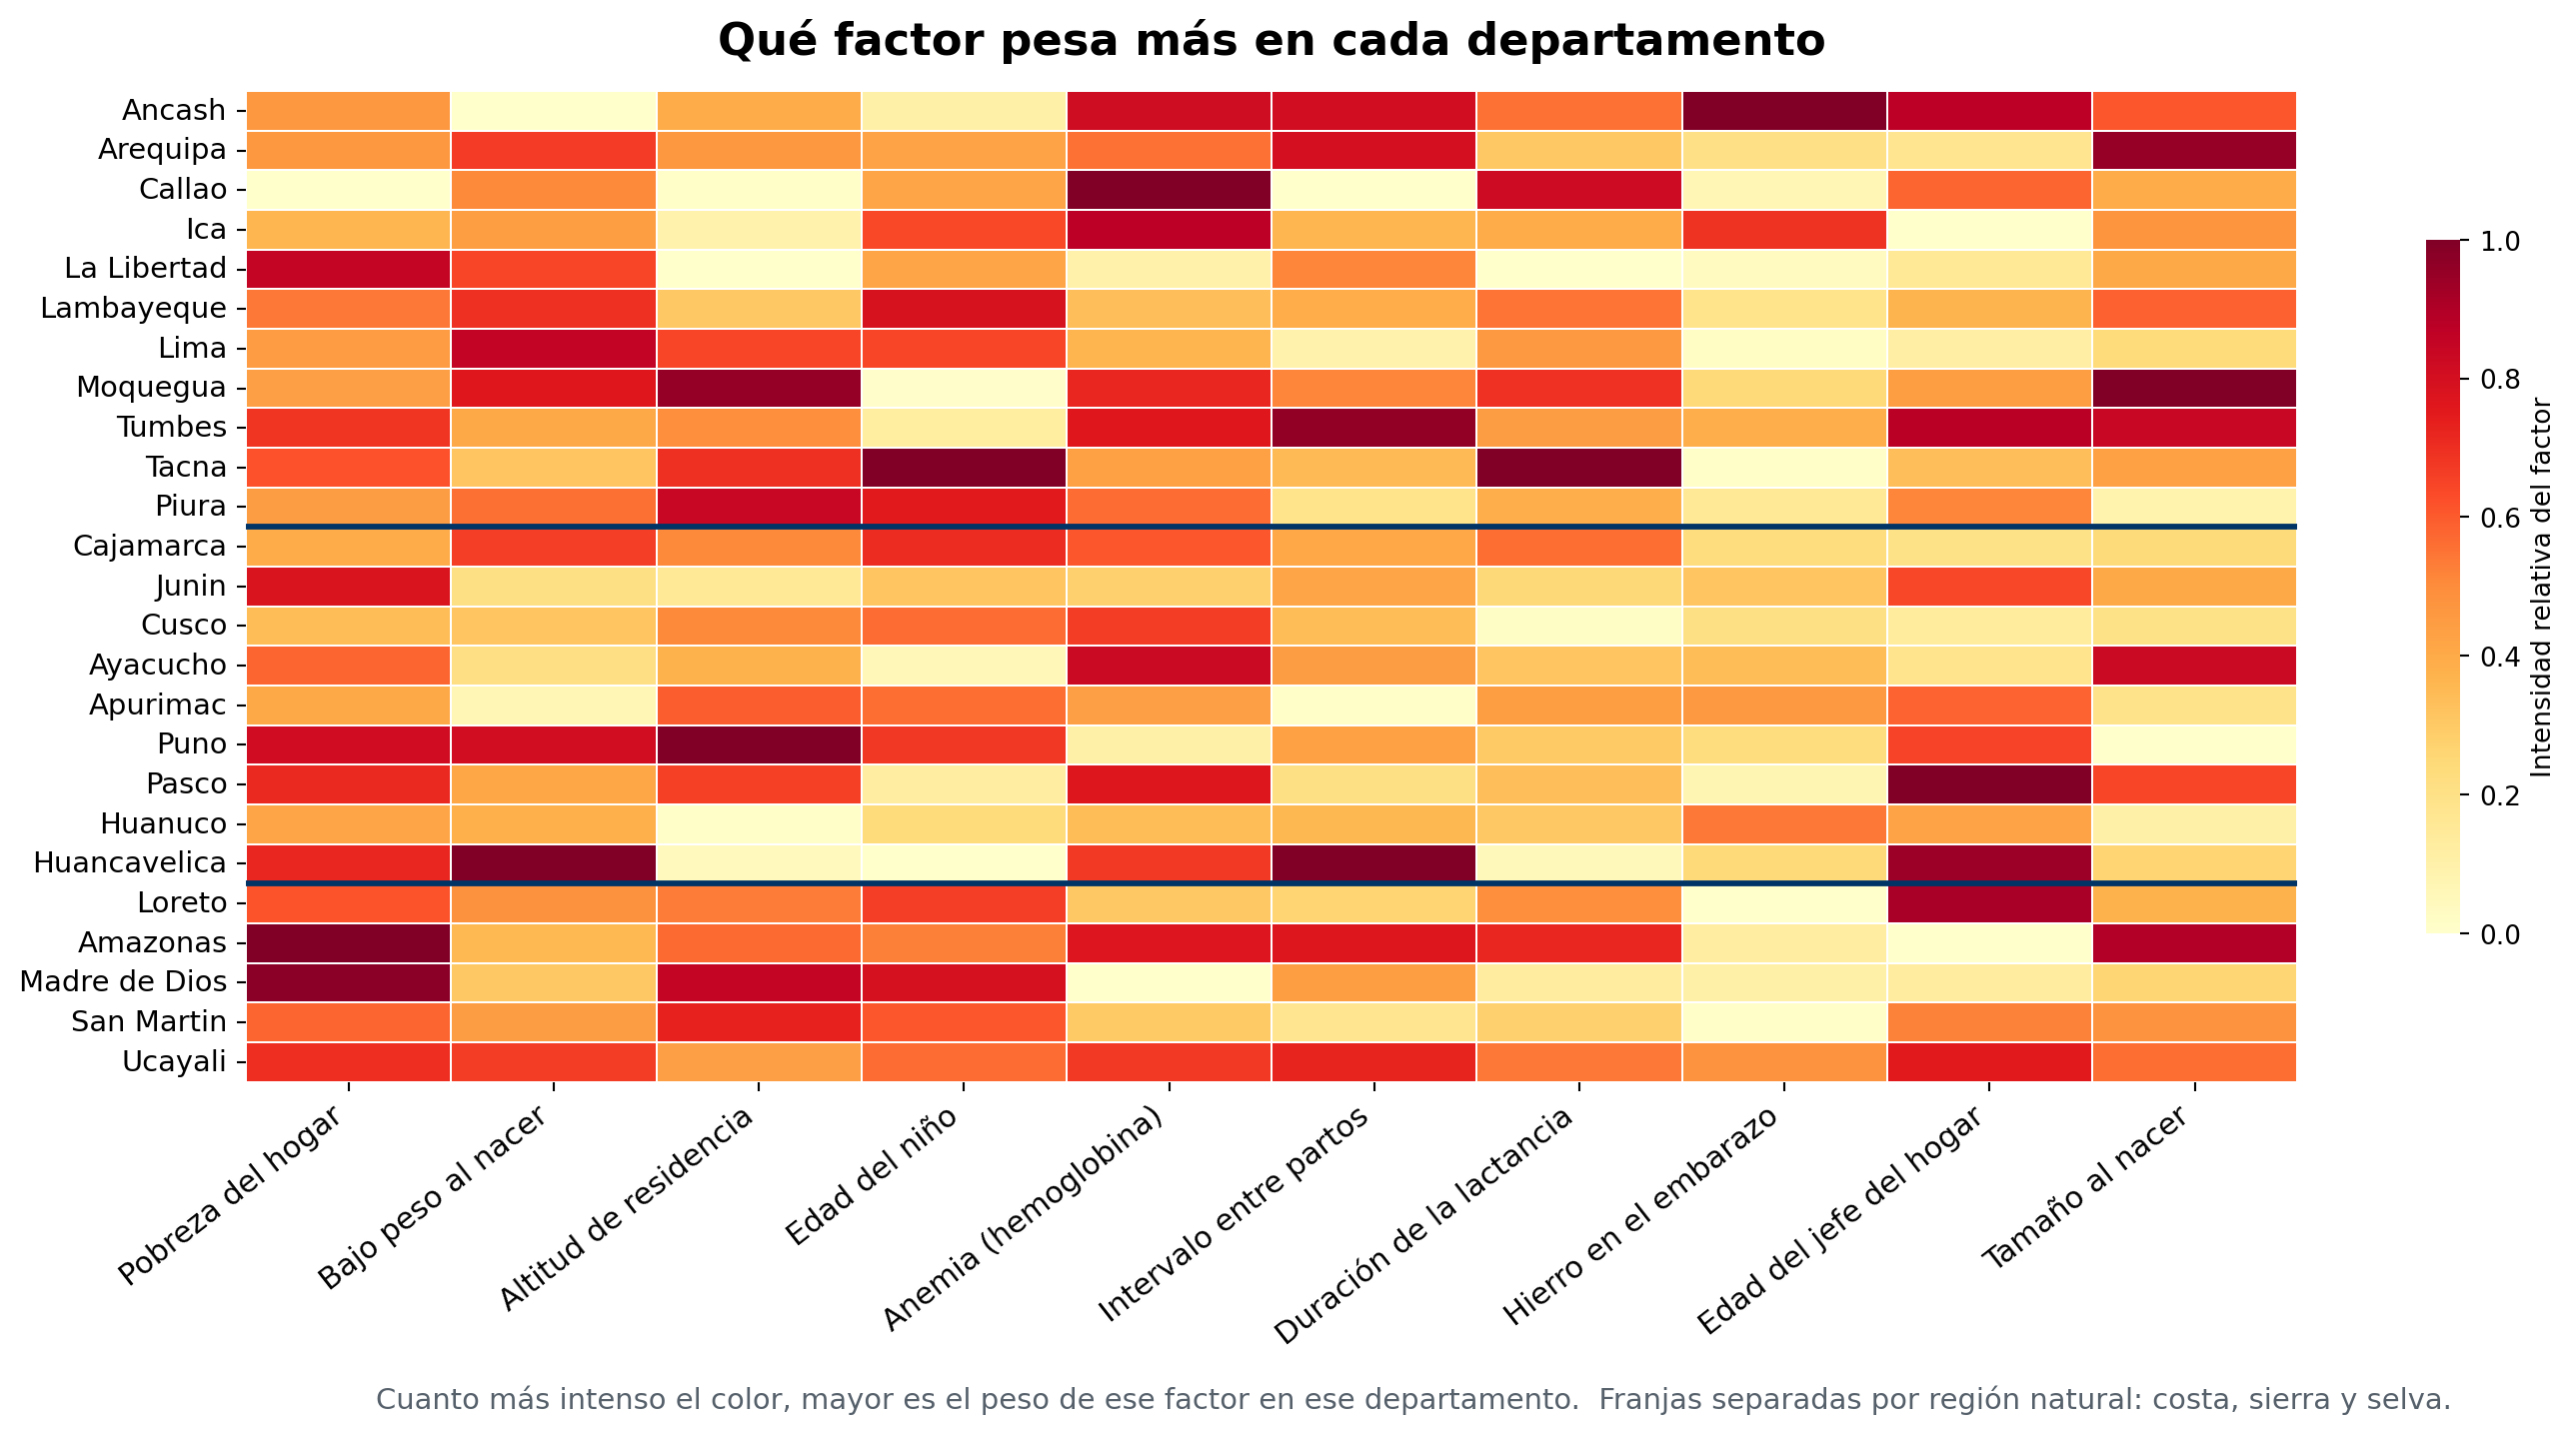
\includegraphics[width=0.9\textwidth]{prism-uploads/Figura9_mapa_factores_departamentos.png}
\caption{Peso relativo de los diez principales factores del modelo en cada departamento (0 = menor peso entre departamentos; 1 = mayor peso), agrupados por región natural.}
\label{fig:mapa_factores}
\end{figure*}

\FloatBarrier
\subsection{Evaluación de la pertinencia por el panel}

Respondieron la ficha cuatro especialistas (tres nutricionistas y un enfermero; Costa y Selva; entre 10 y 20 años de experiencia asistencial). Todos los constructos alcanzaron una mediana igual o superior a 4 (Tabla~\ref{tab:panel}) y la valoración global tuvo una mediana de 9 sobre 10. Los puntos con menor acuerdo fueron la confianza en que los niveles de riesgo asignados son acertados y la disponibilidad en los registros de los datos solicitados y de la hemoglobina, con un evaluador en el puntaje 3 en cada caso (75~\% de acuerdo). Con cuatro evaluadores no se estimaron la confiabilidad ni las relaciones entre constructos: los resultados describen la percepción del panel y no son generalizables.

Las respuestas abiertas coincidieron en cuatro temas: la vigencia de los datos y la equivalencia de las variables entre años, planteada por los cuatro evaluadores; la ampliación a la malnutrición por exceso y a las deficiencias de micronutrientes; un mayor detalle territorial, por ciudad o establecimiento, con retroalimentación de datos locales; y la incorporación de variables adicionales, como la lactancia exclusiva, el consumo de alimentos y las enfermedades crónicas.

\begin{table}[!t]
\centering
\caption{Valoración del panel por constructo (cuatro evaluadores; escala de 1 a 5). Mediana, rango intercuartílico (RIC) y porcentaje de acuerdo (respuestas 4 y 5).}
\label{tab:panel}
\begin{tabular}{lccc}
\hline
Constructo & Mediana & RIC & Acuerdo \\
\hline
Relevancia para el trabajo & 4 & 4--5 & 100~\% \\
Calidad del resultado & 4 & 4--4 & 88~\% \\
Demostrabilidad del resultado & 4.5 & 4--5 & 100~\% \\
Utilidad percibida & 4 & 4--4.25 & 100~\% \\
Facilidad de uso percibida & 4 & 4--5 & 100~\% \\
Condiciones para su uso & 4.5 & 4--5 & 83~\% \\
Respaldo del entorno & 4.5 & 4--5 & 100~\% \\
Intención de uso & 4.5 & 4--5 & 100~\% \\
\hline
Valoración global (1 a 10) & 9 & 8--10 & --- \\
\hline
\end{tabular}
\end{table}

\FloatBarrier
\section{Discusión}

\section{Conclusiones}

\FloatBarrier
\section*{Agradecimientos}
\bibliographystyle{elsarticle-harv} 
\bibliography{example}

%% else use the following coding to input the bibitems directly in the
%% TeX file.

%%\begin{thebibliography}{00}

%% \bibitem[Author(year)]{label}
%% For example:

%% \bibitem[Aladro et al.(2015)]{Aladro15} Aladro, R., Martín, S., Riquelme, D., et al. 2015, \aas, 579, A101


%%\end{thebibliography}

\end{document}

\endinput
%%
%% End of file `elsarticle-template-harv.tex'.
